\documentclass[twoside]{ltjsreport}
\usepackage{silence}
\WarningFilter{caption}{Unknown document}
\usepackage[top=20truemm,bottom=20truemm,left=15truemm,right=15truemm,headheight=20pt]{geometry}
\usepackage{fancyhdr,lastpage,abstract,listings,float,wrapfig,tabularx,multirow,multicol}
\usepackage{hyperref,graphics,graphicx,framed,subcaption}
\usepackage[symbol]{footmisc}
\usepackage{amsmath,amssymb}
\usepackage{tikz}
\usetikzlibrary{calc,arrows.meta,fit,positioning,math}
\newcolumntype{A}{>{\centering\bfseries}X}
\newcolumntype{B}{>{\centering\bfseries\arraybackslash}X}
\newcolumntype{C}{>{\centering\arraybackslash}X}
\newcolumntype{R}{>{\raggedright\arraybackslash}X}
\newcolumntype{L}{>{\raggedleft\arraybackslash}X}
\bibliographystyle{junsrt}
\hypersetup{
    colorlinks=true,
    citecolor=black,
    linkcolor=black,
    urlcolor=black
}
\renewcommand{\chaptermark}[1]{\markboth{第\ \thechapter\ 章\,\, #1}{}}
\fancypagestyle{report}{
    \fancyhf{}
    \fancyhead[RO,LE]{\leftmark}
    \fancyfoot[RO,LE]{\thepage\ /\ \pageref{LastPage}}
    \pagenumbering{arabic}
    }
\fancypagestyle{appendixstyle}{
    \fancyhf{}
    \fancyhead[RO,LE]{付録}
    \fancyfoot[RO,LE]{\thepage\ /\ \pageref{LastPage}}
    \renewcommand{\headrulewidth}{0mm}
}
\lstset{
    language = {Matlab},
    %backgroundcolor={\color[gray]{.90}},
    breaklines = true,
    breakindent = 10pt,
    basicstyle = \ttfamily\small,
    commentstyle = {\ttfamily \color[cmyk]{1,0.4,1,0}},
    classoffset = 0,
    keywordstyle = {\bfseries \color[cmyk]{0,1,0,0}},
    stringstyle = {\ttfamily \color[rgb]{0,0,1}},
    frame = left,
    %他オプション:leftline,topline,bottomline,lines,single,shadowbox
    framesep = 5pt,
    numbers = none,
    stepnumber = 1,
    numberstyle = \small,
    tabsize = 4,
    captionpos = t,
    otherkeywords = {xticks, yticks, exportgraphics, imwrite, bitshift, uint8, double}
}
\renewcommand{\figurename}{図}
\renewcommand{\tablename}{表}
\renewcommand{\lstlistingname}{src.}
\renewcommand{\thefootnote}{\fnsymbol{footnote}}
\renewcommand{\contentsname}{目次}
\renewcommand{\listfigurename}{図目次}
\renewcommand{\listtablename}{表目次}
\renewcommand{\lstlistlistingname}{ソースコード}
\renewcommand{\thefigure}{\thechapter-\arabic{figure}}
\renewcommand{\thetable}{\thechapter-\arabic{table}}
\renewcommand{\theequation}{\thechapter.\arabic{equation}}
\renewcommand{\thesubfigure}{(\alph{subfigure})}
\renewcommand{\labelenumi}{\textbf{\theenumi}.\ }
\renewcommand{\eqref}[1]{式(\ref{#1})}
\newcommand{\matlab}{\text{{\large M}ATLAB\raisebox{2mm}{\tiny\textregistered}}}
\newcommand{\mat}[2]{\(#1\)行\(#2\)列}
\newcommand{\figref}[1]{図\ref{#1}}
\newcommand{\tblref}[1]{表\ref{#1}}
\newcommand{\srcref}[1]{src.\ref{#1}}
\newcommand{\scall}[1]{課題\ (#1)\ のスクリプトは,}
\newcommand{\sref}[1]{\(\underset{\blacktriangleright\textrm{p.\pageref{#1}}}{\textrm{\srcref{#1}}}\)}
\captionsetup[subfigure]{labelformat=simple}
\makeatletter
\@addtoreset{figure}{chapter}
\@addtoreset{table}{chapter}
\@addtoreset{lstlisting}{chapter}
\@addtoreset{footnote}{page}
\renewcommand{\chapter}{%
    \if@openright\cleardoublepage\else\clearpage\fi
    \global\@topnum\z@
    \secdef\@chapter\@schapter}
\makeatother
\AtBeginDocument{
    \renewcommand{\thelstlisting}{\thechapter-\arabic{lstlisting}}
}
\title{{\normalsize 情報学群実験第3C/3i 実験レポート 第2回}\\Title}
\author{1250373\hspace{1\zw}溝口 洸熙\thanks{高知工科大学 情報学群 情報セキュリティシステム研究室}\\Group 10}
\date{May 7th, 2023}
\begin{document}
% paragraph command
\newcommand{\purpose}{\subsection{実験の目的}}
\newcommand{\method}{\subsection{実験の方法と考え方}}
\newcommand{\result}{\subsection{実験の結果}}
\newcommand{\consideration}{\subsection{考察}}
\newcommand{\conclusion}{\subsection{結論}}
% 課題1
\newcommand{\kadaiaa}{カラーチャネル操作}
\newcommand{\kadaiab}{画像の量しかビット数変換}
\newcommand{\kadaiac}{階調反転}
\newcommand{\kadaiad}{閾値処理}
\newcommand{\kadaiae}{ヒストグラム}
% 課題2
\newcommand{\kadaiba}{テスト画像作成}
\newcommand{\kadaibb}{平滑化フィルタ・メディアンフィルタ}
\newcommand{\kadaibc}{微分フィルタ}
\newcommand{\kadaibd}{ラプラシアンフィルタ}
\newcommand{\kadaibe}{色空間変換}
\maketitle
\renewcommand{\abstractname}{概要}
\begin{abstract}
    本実験では,画像情報処理,視覚情報処理を扱う.画像情報処理では,カラーチャネル操作や閾値処理,量子化数変換などの基礎的な画像処理を行い,それらの技術を用いて画像フィルタや背景差分画像の作成や肌色領域の抽出,2次元フーリエ変換を行う.2次元フーリエ変換のパワースペクトルと原画像の関係や,2次元フーリエ変換後の出力と,画像座標との関係が明らかになった.また,背景差分画像と色空間変換後の肌色領域抽出で,対象物の抽出における特徴も明らかとなった.
    視覚情報処理では,方位残効を扱う.\matlab 上で方位残効刺激を作成する.この実験より,縞模様方位の大きさと,方位残効の度合いの関係を,ヒトの視覚情報処理を考慮した上で明らかになった.
\end{abstract}
\pagenumbering{roman}\thispagestyle{plain}
\tableofcontents
\listoffigures
\listoftables
\lstlistoflistings
\newpage
\pagestyle{report}
\setcounter{page}{1}
\chapter{\kadaia}
\section{\purpose}
本章では,画像のカラーチャネル操作,量子化,階調反転,閾値処理を行う.またグレイスケール画像に対してヒストグラムを作成する.
\paragraph{\kadaiaa}RGB色空間の画像を,緑チャネルだけを抜き出してグレイスケール画像を作成する.赤チャネル,青チャネルについても同様にグレイスケール画像を生成する.さらに,RGB画像の赤チャネルと青チャネルを入れ替えたカラー画像を作成する.
\paragraph{\kadaiab}グレイスケール画像を生成する.緑チャネルは色の濃淡を多く含む.RGB色空間から色の濃淡を抽出したい場合は,緑(G)の成分を多く抽出するとよい.具体的な割合を,\eqref{equ:grayscale}に示す.ここではNTSC輝度信号を取り出す方法で行う.生成したグレイスケール画像に対して,画像の量子化数を変更することによる,画像の変化を確認する.量子化数は8Bit,4Bit,2Bit,1Bitの4種をテストする.量子化数1Bitの画像を2値画像という.
\begin{align}
    \textrm{Gray scale image} & = \textrm{Red}\times 30\% +\textrm{Green}\times 59\% +\textrm{Blue}\times 11\%\label{equ:grayscale}
\end{align}
\paragraph{\kadaiac}各量子化数の画像に対して,その画像を階調反転させる.階調反転とは,白黒を反転させることである.量子化数による階調変換後の画像を比較する.
\paragraph{\kadaiad}閾値処理とは,とある値(閾値)以上の場合を白,閾値以下を黒とし,2値画像を作成することである.
\paragraph{\kadaiae}量子化数8Bitのグレイスケール画像のヒストグラムを作成する.画素値\(n(n=0,1,\dots ,255)\)の画素が何画素含まれているかのヒストグラムを作成する.
\paragraph{\kadaiaf}自分が写っている写真と,背景だけが写っている写真の差分画像をとる.これを背景差分と呼ぶ.背景差分の後,閾値処理を行う.物体領域を正しく検出するために考慮する点を考察する.
\section{\method}
\paragraph{実験に用いる装置}このレポート内すべての実験にはMathWorks\raisebox{2mm}{\tiny\textregistered}社の\matlab を用いて,\tblref{tbl:実験環境}の環境下で実験する.
\begin{table}[H]
    \caption{実験環境}
    \label{tbl:実験環境}
    \begin{tabularx}{\textwidth}{AR}
        \hline
        実験機                      & MacBook Air 2022 (Apple社)\texttt{MLY13J/A}    \\
        プロセッサ                    & Apple Silicon M2\ \  8コアCPU,8コアGPU            \\
        メモリ                      & 8GB                                           \\
        \multirow{2}{*}{\matlab} & R2023a - academic use (Update1 9.14.02239454) \\
                                 & 64-bit (maci64) March 30, 2023                \\
        \hline
    \end{tabularx}
\end{table}
また,このレポートないすべての実験では\matlab でプロットしたグラフを出力するための\texttt{exportgraphics}関数,画像を書き出すための\texttt{imwrite}関数を用いる(\srcref{src:グラフ・画像出力}).
\begin{lstlisting}[numbers={none},caption={グラフ・画像出力},label={src:グラフ・画像出力}]
exportgraphics(figurename,'path/figure_name.pdf','ContentType','vector');
imwrite(data,"path/figure_name.png");
\end{lstlisting}
\paragraph{\kadaiaa}
\texttt{imwrite}関数を用いて,画像の読み込む.読み込んだ画像はRGB色空間で保存されており,チャネル1にはR,チャネル2にはG,チャネル3にはBが保存されている.
グレイスケール画像を作成するには,\eqref{equ:grayscale}の割合で画像を加算合成する.\mat{m}{n}の行列\texttt{A}に対して,\mat{1}{n}を取り出したければ,\verb|A(1,:)|と記述する.\verb|:|は,すべての要素を表す記号である.
赤チャネルと青チャネルを入れ替えるためには,赤チャネルの行列と青チャネルの行列を変数に保存し,それぞれ互いのチャネルに代入する.\scall{\kadaiaa}\sref{src:05_01}.

\begin{wrapfigure}{r}[0mm]{.3\textwidth}
    \centering
    \vspace{-.7cm}
    \begin{lstlisting}[caption={\texttt{bitshift}関数},label={src:bitshift}]
img = bitshift(img, n);
    \end{lstlisting}
    \vspace{-.5cm}
\end{wrapfigure}
\paragraph{\kadaiab}
量子化数を変更するために,\texttt{bitshift}関数を用いる(\srcref{src:bitshift}).
この関数は,\texttt{img}を左に\texttt{n}ビットシフトする関数である.右シフトしたい場合は\texttt{n}を負の数で与える.
ビットシフトについて,1ビット右シフトするごとにそのデータは\(1/2\)される.
これを利用して,量子化数4Bitの場合は右に4Bitシフト,量子化数2Bitの場合は右に6Bitシフト,量子化数1Bitの場合は右に7Bitシフトする.

\begin{wrapfigure}{r}[0mm]{.225\textwidth}
    \centering
    \vspace{-.5cm}
    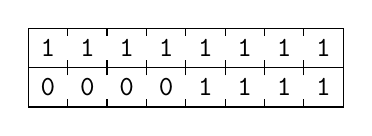
\begin{tikzpicture}
        \coordinate (A) at (4,1);
        \draw (0,0.5)--(4,0.5);
        \draw (0,0)rectangle(A);
        \foreach \x in {1,2,...,8}
            {
                \draw (\x/2,0.4)--(\x/2,0.6);
                \draw (\x/2,1)--(\x/2,0.9);
                \draw (\x/2,0)--(\x/2,0.1);
                \node at ($(\x/2-1/2,0.5)!0.5!(\x/2,1)$){\texttt{1}};
                \node at ($(\x/2-1/2,0)!0.5!(\x/2,0.5)$){\ifnum\x<5\texttt{0}\else\ifnum\x>5\texttt{1}\else\ifnum\x=5\texttt{1}\fi\fi\fi};
            }
    \end{tikzpicture}
    \caption{4ビットシフト}
    \label{fig:4ビットシフト}
    \vspace{-.5cm}
\end{wrapfigure}
量子化数4Bitを例にあげる.仮に画素値が\texttt{255}(白)を持つ画素の場合,量子化数を4Bitにする,つまり4Bit右シフトすると,画素値は\texttt{15}になる(\figref{fig:4ビットシフト}).このままでは画素値の範囲が\(0\)から\(15\)となる.
この対策として,全体画素値と\(255/15\)の積を取ることで,画素値を\(0\)から\(255\)にスケーリングする.\scall{\kadaiab}\sref{src:05_02}.
\paragraph{\kadaiac}
各量子化数ごとに階調反転する.階調反転を実現するためには,階調反転した画像を\texttt{double}型に変換したあと,\(-1\)との積をとり,\(255\)を足した後で\texttt{unit8}型に変換する\footnote{その画像の各画素値が\texttt{double}型であるとき,\texttt{imwrite}が,データを自動的にリスケールし書き出すため.}.\scall{\kadaiac}\sref{src:05_03}.

\begin{wrapfigure}{r}[0mm]{.3\textwidth}
    \centering
    \vspace{-.7cm}
    \begin{lstlisting}[caption={判定結果の格納},label={src:判定結果の格納}]
mat = [1 2 3; 4 5 6; 7 8 9];
bin = mat > 5;
% -- 結果 --
bin = [0 0 0; 0 0 1; 1 1 1];     
    \end{lstlisting}
    \vspace{-.5cm}
\end{wrapfigure}
\paragraph{\kadaiad}
\matlab には,判定結果のブール値を行列に格納する機能がある.
\srcref{src:判定結果の格納}より,行列\texttt{mat}の各元が\(5\)より大きい箇所を\(1\),\(5\)以下のところを\(0\)とする行列\texttt{bin}を作成できる.この行列を真理行列と呼ぶ.
この機能を用いて,ある閾値に対して,閾値よりも大きければ\(1\)を戻し,閾値以下であれば\(0\)を戻す行列を作成する.画素値の範囲を\(0\)から\(255\)へするために,行列の各元と\(255\)の積をとる.今回は,閾値を\(64\),\(128\),\(192\)で実験する.\scall{\kadaiad}\sref{src:05_04}

\begin{wrapfigure}{r}[0mm]{.3\textwidth}
    \centering
    \vspace{-.9cm}
    \begin{lstlisting}[caption={\texttt{sum}関数},label={src:sum関数}]
matA = [1 2 3];
s_matA = sum(matA); 
% -> 出力:6
matB = [1 2; 1 1; 1 1];
s_matB = sum(matB); 
% -> 出力:[3 4]
s_s_matB = sum(sum(matB)); 
% -> 出力:12
    \end{lstlisting}
    \vspace{-.7cm}
\end{wrapfigure}
\paragraph{\kadaiae}
ヒストグラムを作成するために,この関数は行列の元を足し合わせる\texttt{sum}関数を用いる(\srcref{src:sum関数}).
各画素値\(0\)から\(255\)に対して,その画素値と等しい箇所を\(1\)とする真理行列を作成し,各元の和を\texttt{sum}関数を用いて算出する.
その結果が,ある画素値がいくつ画像に含まれているかを指す.
\paragraph{\kadaiaf}
固定カメラ\footnote{手での固定は,背景がズレる可能性があるので,カメラを固定して撮影した.}で撮影した写真を用いる.「背景と被写体が写っている画像\texttt{img\_sbj}」「背景のみの画像\texttt{img\_bg}」の2点を撮影した.背景差分画像は,\(\texttt{img\_sbj}-\texttt{img\_bg}\)で生成する.
生成した画像に対して,閾値処理する.閾値処理する前後での画像比較,閾値による比較し,考察する.今回,閾値を\(32\),\(64\),\(128\)で実験する.\scall{\kadaiaf}\sref{src:05_06}.
\section{\result}
\begin{figure}[h]
    \newcommand{\vsp}{\vspace{2em}}
    \centering
    \begin{minipage}[b]{.19\textwidth}
        \centering
        
\includegraphics[keepaspectratio,width=\textwidth]{../../kut.jpg}
        \subcaption{元画像}
        \label{fig:元画像}
    \end{minipage}
    \begin{minipage}[b]{.19\textwidth}
        \centering
        
\includegraphics[keepaspectratio,width=\textwidth]{../../Figures/05_11_r.png}
        \subcaption{赤チャネル}
    \end{minipage}
    \begin{minipage}[b]{.19\textwidth}
        \centering
        
\includegraphics[keepaspectratio,width=\textwidth]{../../Figures/05_12_g.png}
        \subcaption{緑チャネル}
    \end{minipage}
    \begin{minipage}[b]{.19\textwidth}
        \centering
        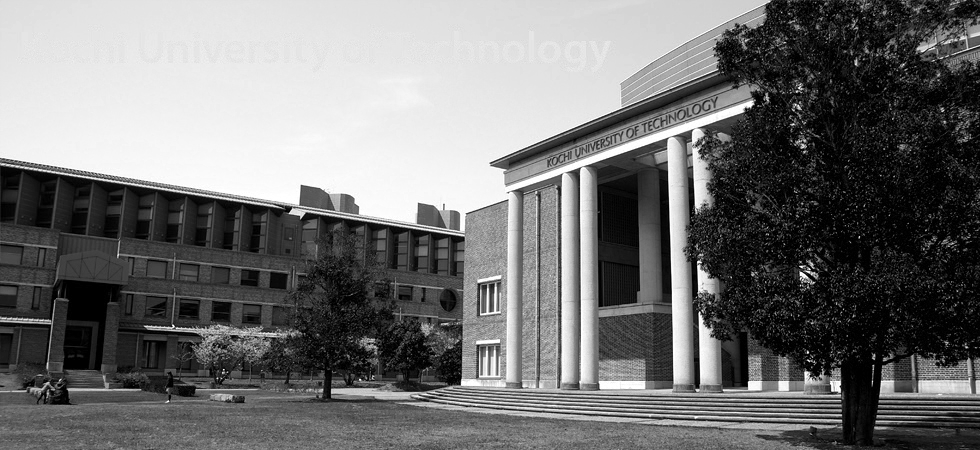
\includegraphics[keepaspectratio,width=\textwidth]{../../Figures/05_13_b.png}
        \subcaption{青チャネル}
    \end{minipage}
    \begin{minipage}[b]{.19\textwidth}
        \centering
        
\includegraphics[keepaspectratio,width=\textwidth]{../../Figures/05_14_change.png}
        \subcaption{赤青チャネル入れ替え}
    \end{minipage}
    \caption{\kadaiaa\ 実験結果}
    \vsp
    \begin{minipage}[b]{.23\textwidth}
        \centering
        
\includegraphics[keepaspectratio,width=\textwidth]{../../Figures/05_21_gimg.png}
        \subcaption{量子化数\ 8Bit\footnotemark[1]}
    \end{minipage}
    \begin{minipage}[b]{.23\textwidth}
        \centering
        
\includegraphics[keepaspectratio,width=\textwidth]{../../Figures/05_22_4bit.png}
        \subcaption{量子化数\ 4Bit}
    \end{minipage}
    \begin{minipage}[b]{.23\textwidth}
        \centering
        
\includegraphics[keepaspectratio,width=\textwidth]{../../Figures/05_23_2bit.png}
        \subcaption{量子化数\ 2Bit}
    \end{minipage}
    \begin{minipage}[b]{.23\textwidth}
        \centering
        
\includegraphics[keepaspectratio,width=\textwidth]{../../Figures/05_24_1bit.png}
        \subcaption{量子化数\ 1Bit}
    \end{minipage}
    \caption{\kadaiab\ 実験結果}
    \vsp
    \begin{minipage}[b]{.23\textwidth}
        \centering
        
\includegraphics[keepaspectratio,width=\textwidth]{../../Figures/05_31_8.png}
        \subcaption{量子化数\ 8Bit}
    \end{minipage}
    \begin{minipage}[b]{.23\textwidth}
        \centering
        
\includegraphics[keepaspectratio,width=\textwidth]{../../Figures/05_32_4.png}
        \subcaption{量子化数\ 4Bit}
    \end{minipage}
    \begin{minipage}[b]{.23\textwidth}
        \centering
        
\includegraphics[keepaspectratio,width=\textwidth]{../../Figures/05_33_2.png}
        \subcaption{量子化数\ 2Bit}
    \end{minipage}
    \begin{minipage}[b]{.23\textwidth}
        \centering
        
\includegraphics[keepaspectratio,width=\textwidth]{../../Figures/05_34_1.png}
        \subcaption{量子化数\ 1Bit}
    \end{minipage}
    \caption{\kadaiac\ 実験結果}
    \vsp
    \begin{minipage}[b]{.7\textwidth}
        \centering
        \begin{minipage}[b]{.3\textwidth}
            \centering
            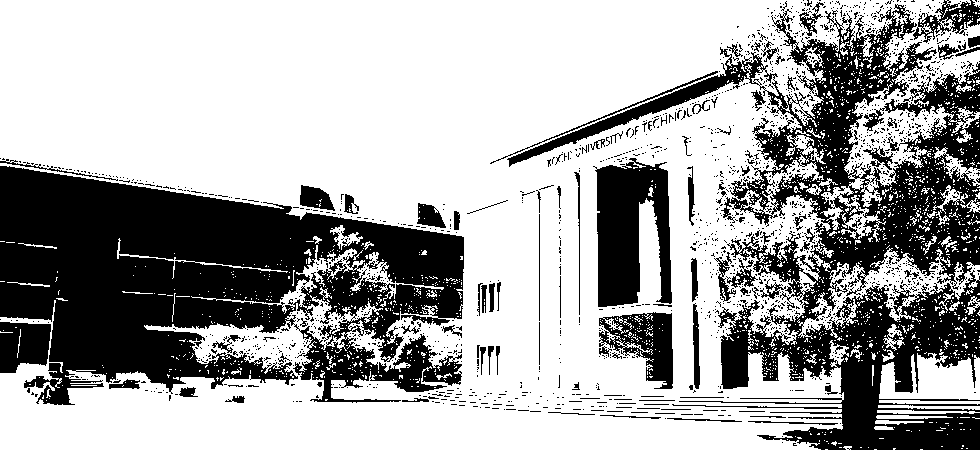
\includegraphics[keepaspectratio,width=\textwidth]{../../Figures/05_41.png}
            \subcaption{閾値\ \(64\)}
        \end{minipage}
        \begin{minipage}[b]{.3\textwidth}
            \centering
            
\includegraphics[keepaspectratio,width=\textwidth]{../../Figures/05_42.png}
            \subcaption{閾値\ \(128\)}
        \end{minipage}
        \begin{minipage}[b]{.3\textwidth}
            \centering
            
\includegraphics[keepaspectratio,width=\textwidth]{../../Figures/05_43.png}
            \subcaption{閾値\ \(192\)}
        \end{minipage}
        \caption{\kadaiad\ 実験結果}
    \end{minipage}
    \begin{minipage}[b]{.25\textwidth}
        \centering
        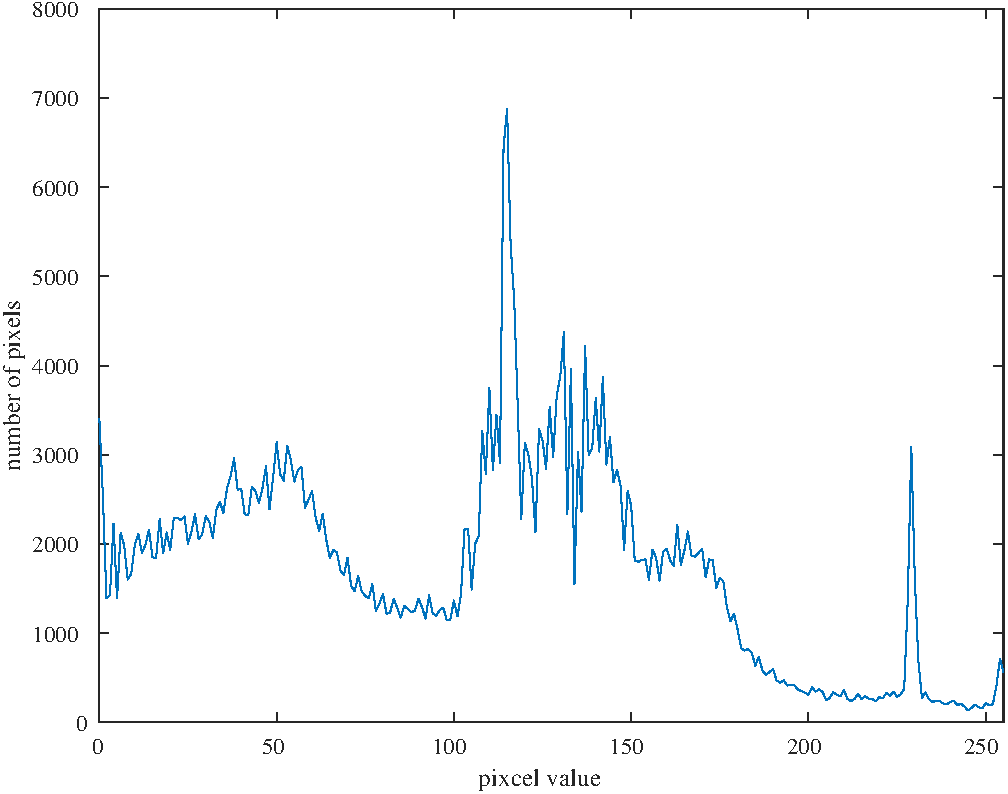
\includegraphics[keepaspectratio,width=\textwidth]{../../Figures/05_50_graph.pdf}
        \caption{\kadaiae\ 実験結果}
    \end{minipage}
    \nextfloat
    \\\vsp
    \begin{minipage}[b]{.49\textwidth}
        \centering
        \begin{minipage}[b]{.3\textwidth}
            \centering
            
\includegraphics[keepaspectratio,width=\textwidth]{../../05_UnderstandingImages/fig1_g.jpg}
            \subcaption{被写体と背景}
        \end{minipage}
        \begin{minipage}[b]{.3\textwidth}
            \centering
            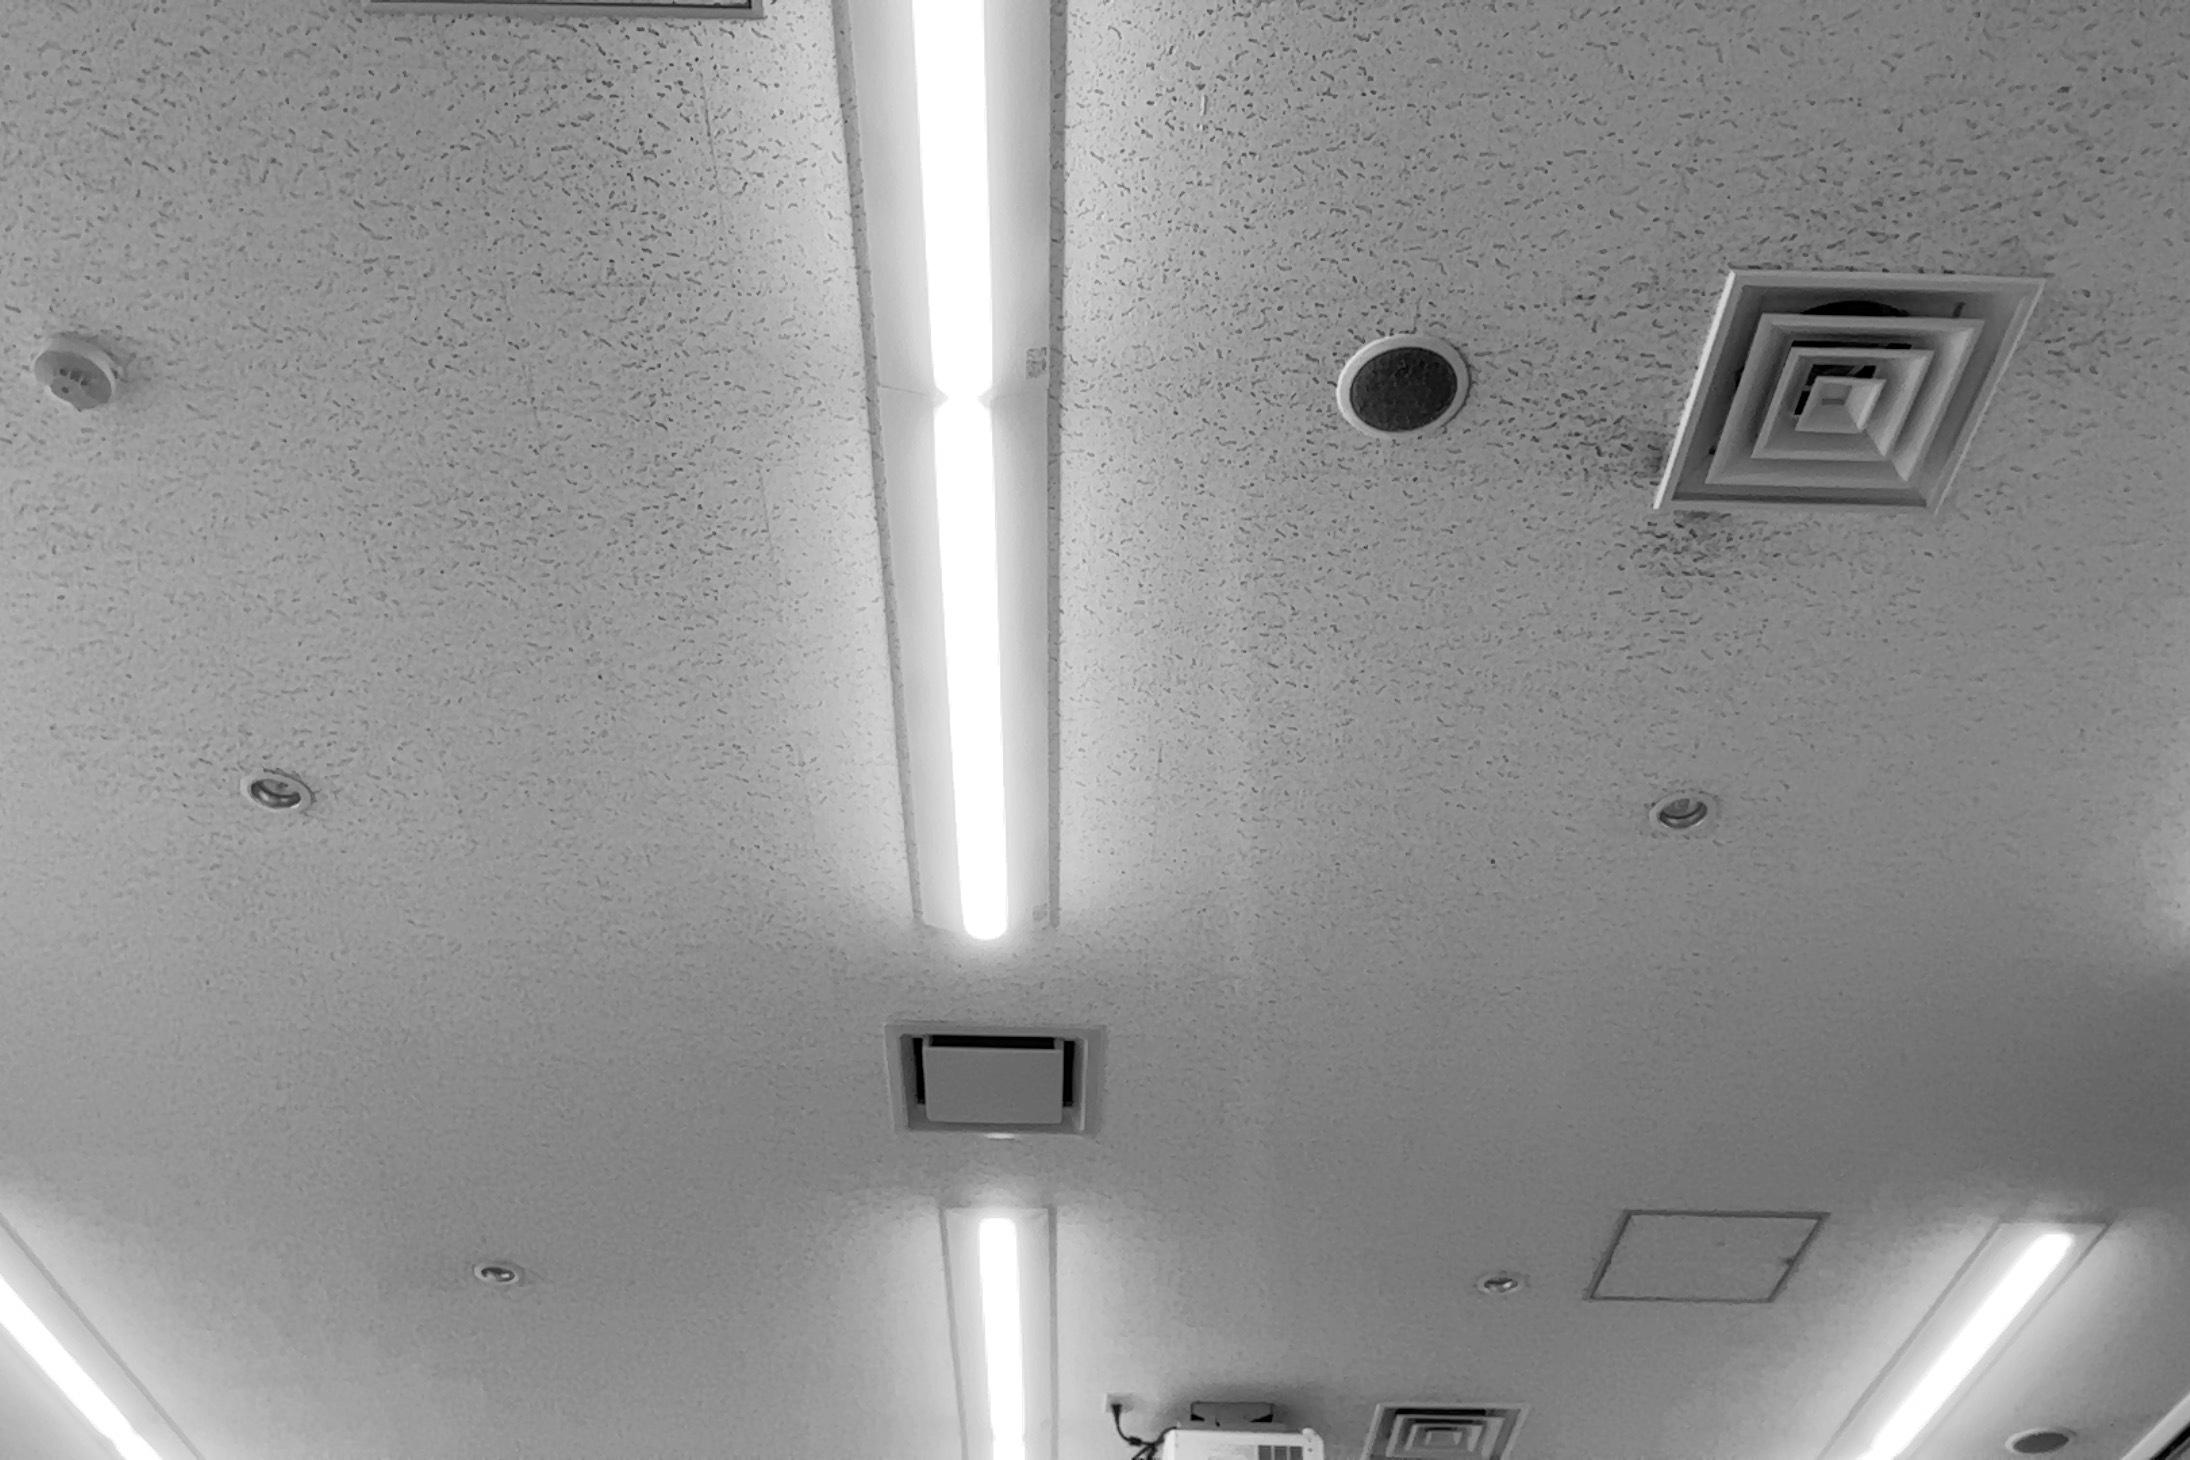
\includegraphics[keepaspectratio,width=\textwidth]{../../05_UnderstandingImages/fig2_g.jpg}
            \subcaption{背景のみ}
        \end{minipage}
        \begin{minipage}[b]{.3\textwidth}
            \centering
            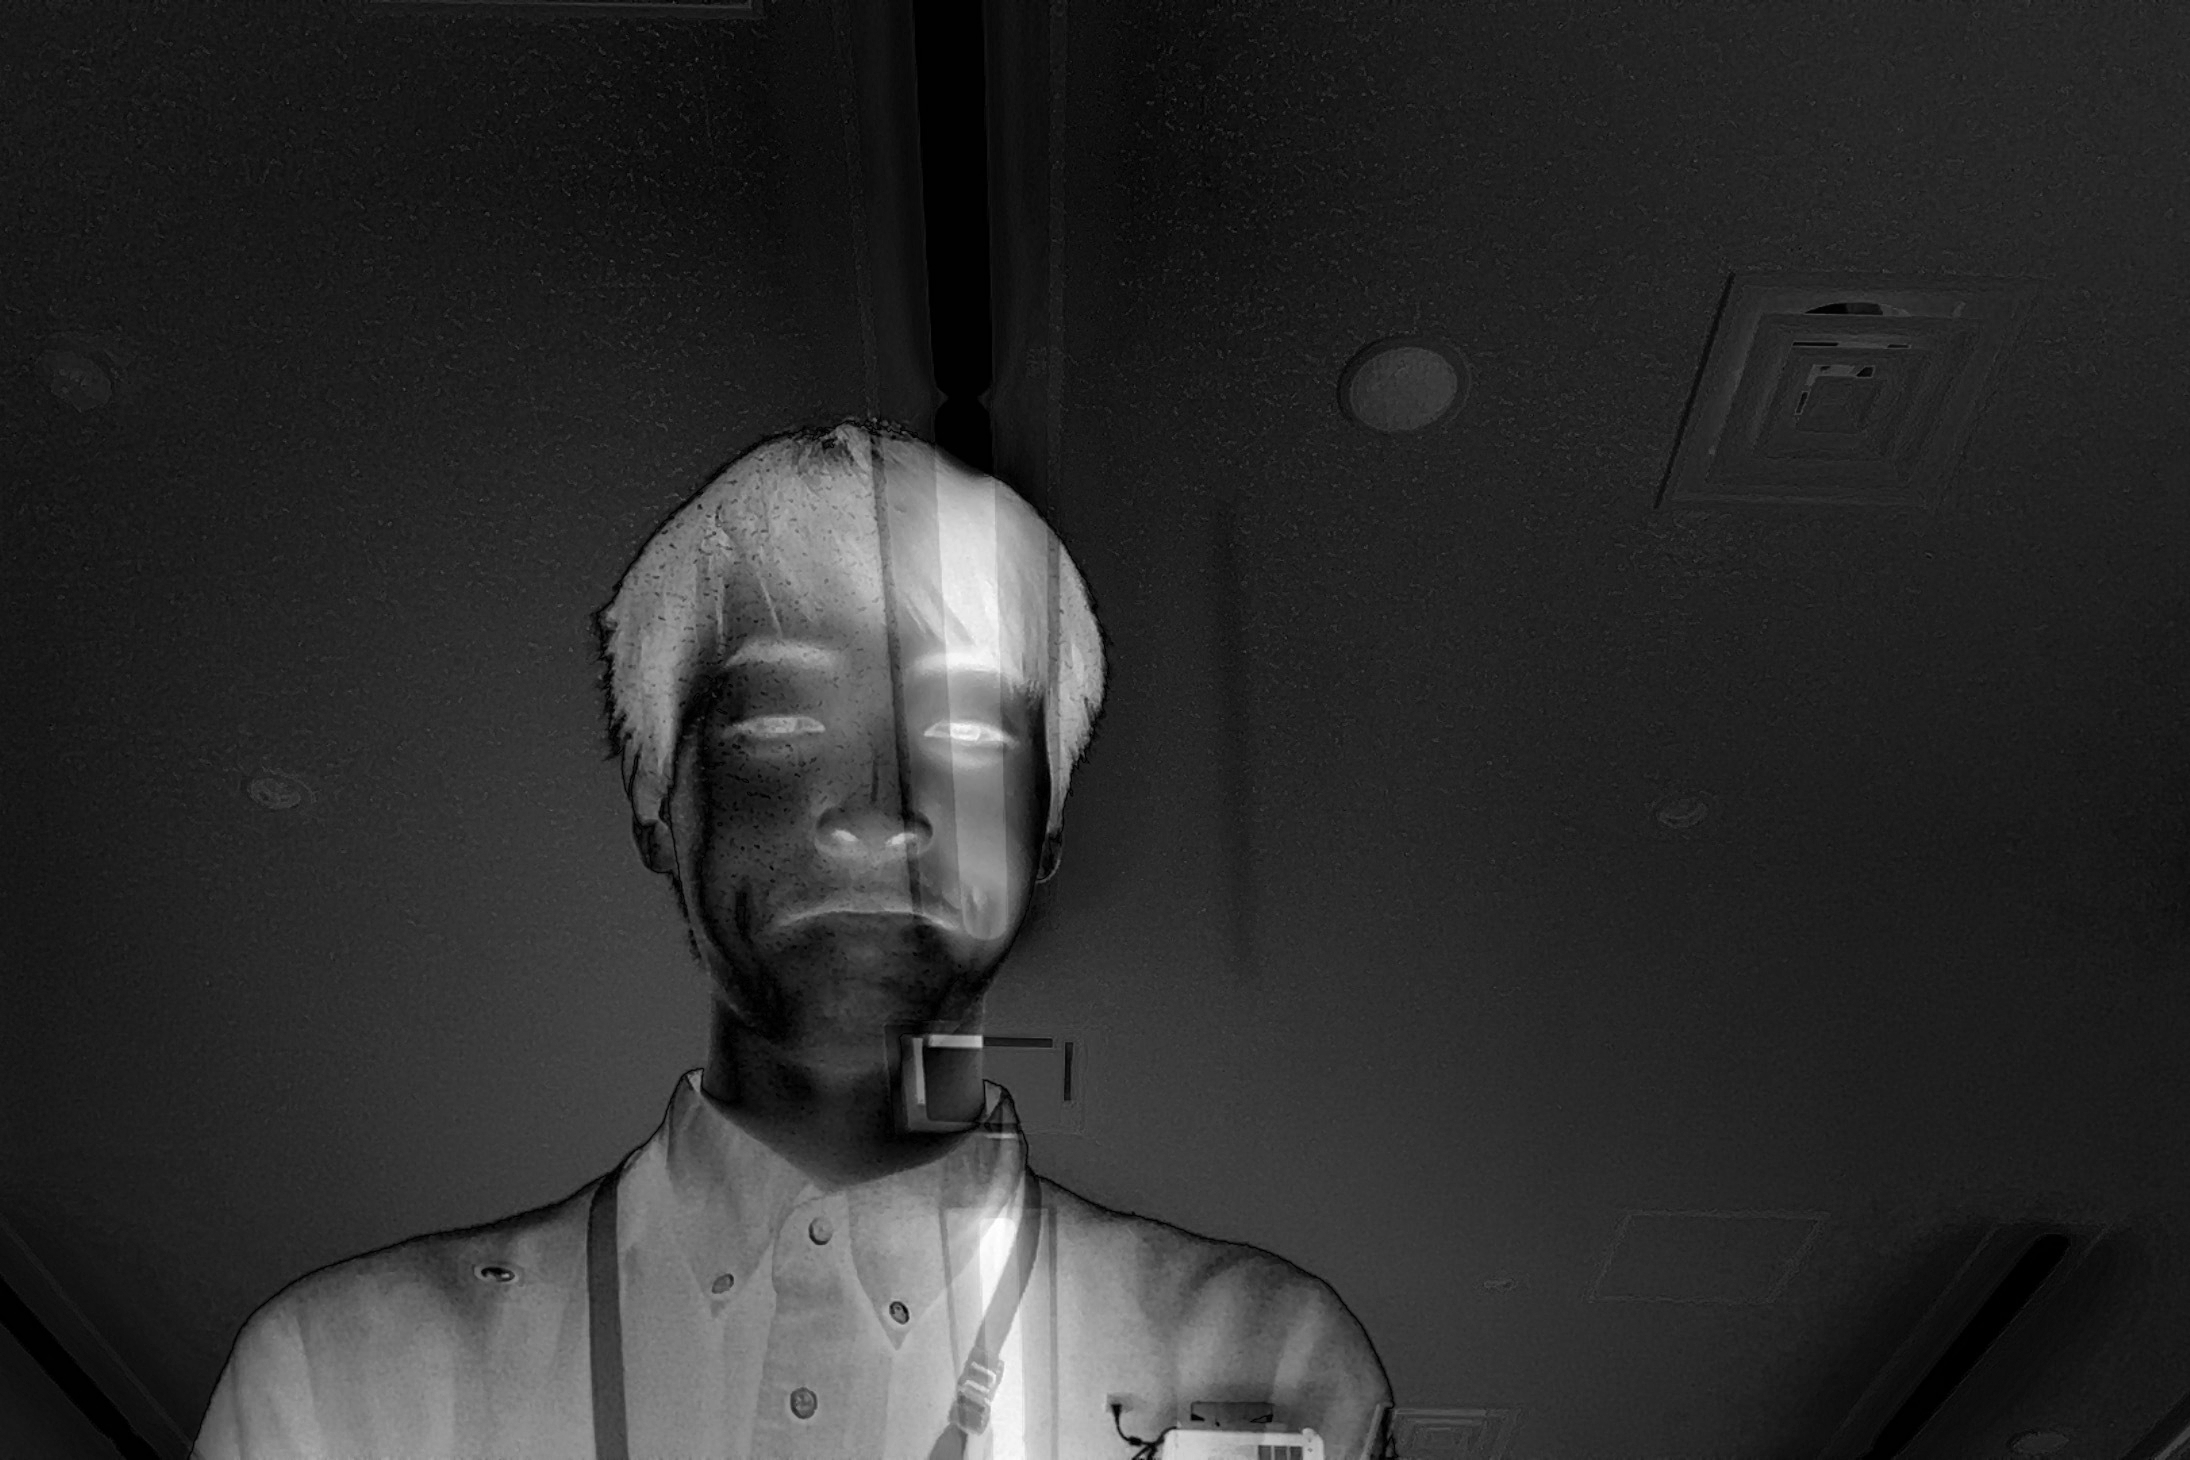
\includegraphics[keepaspectratio,width=\textwidth]{../../Figures/05_60.png}
            \subcaption{背景差分画像}
        \end{minipage}
        \caption{\kadaiaf\ 実験結果}
    \end{minipage}
    \nextfloat
    \begin{minipage}[b]{.49\textwidth}
        \centering
        \begin{minipage}[b]{.3\textwidth}
            \centering
            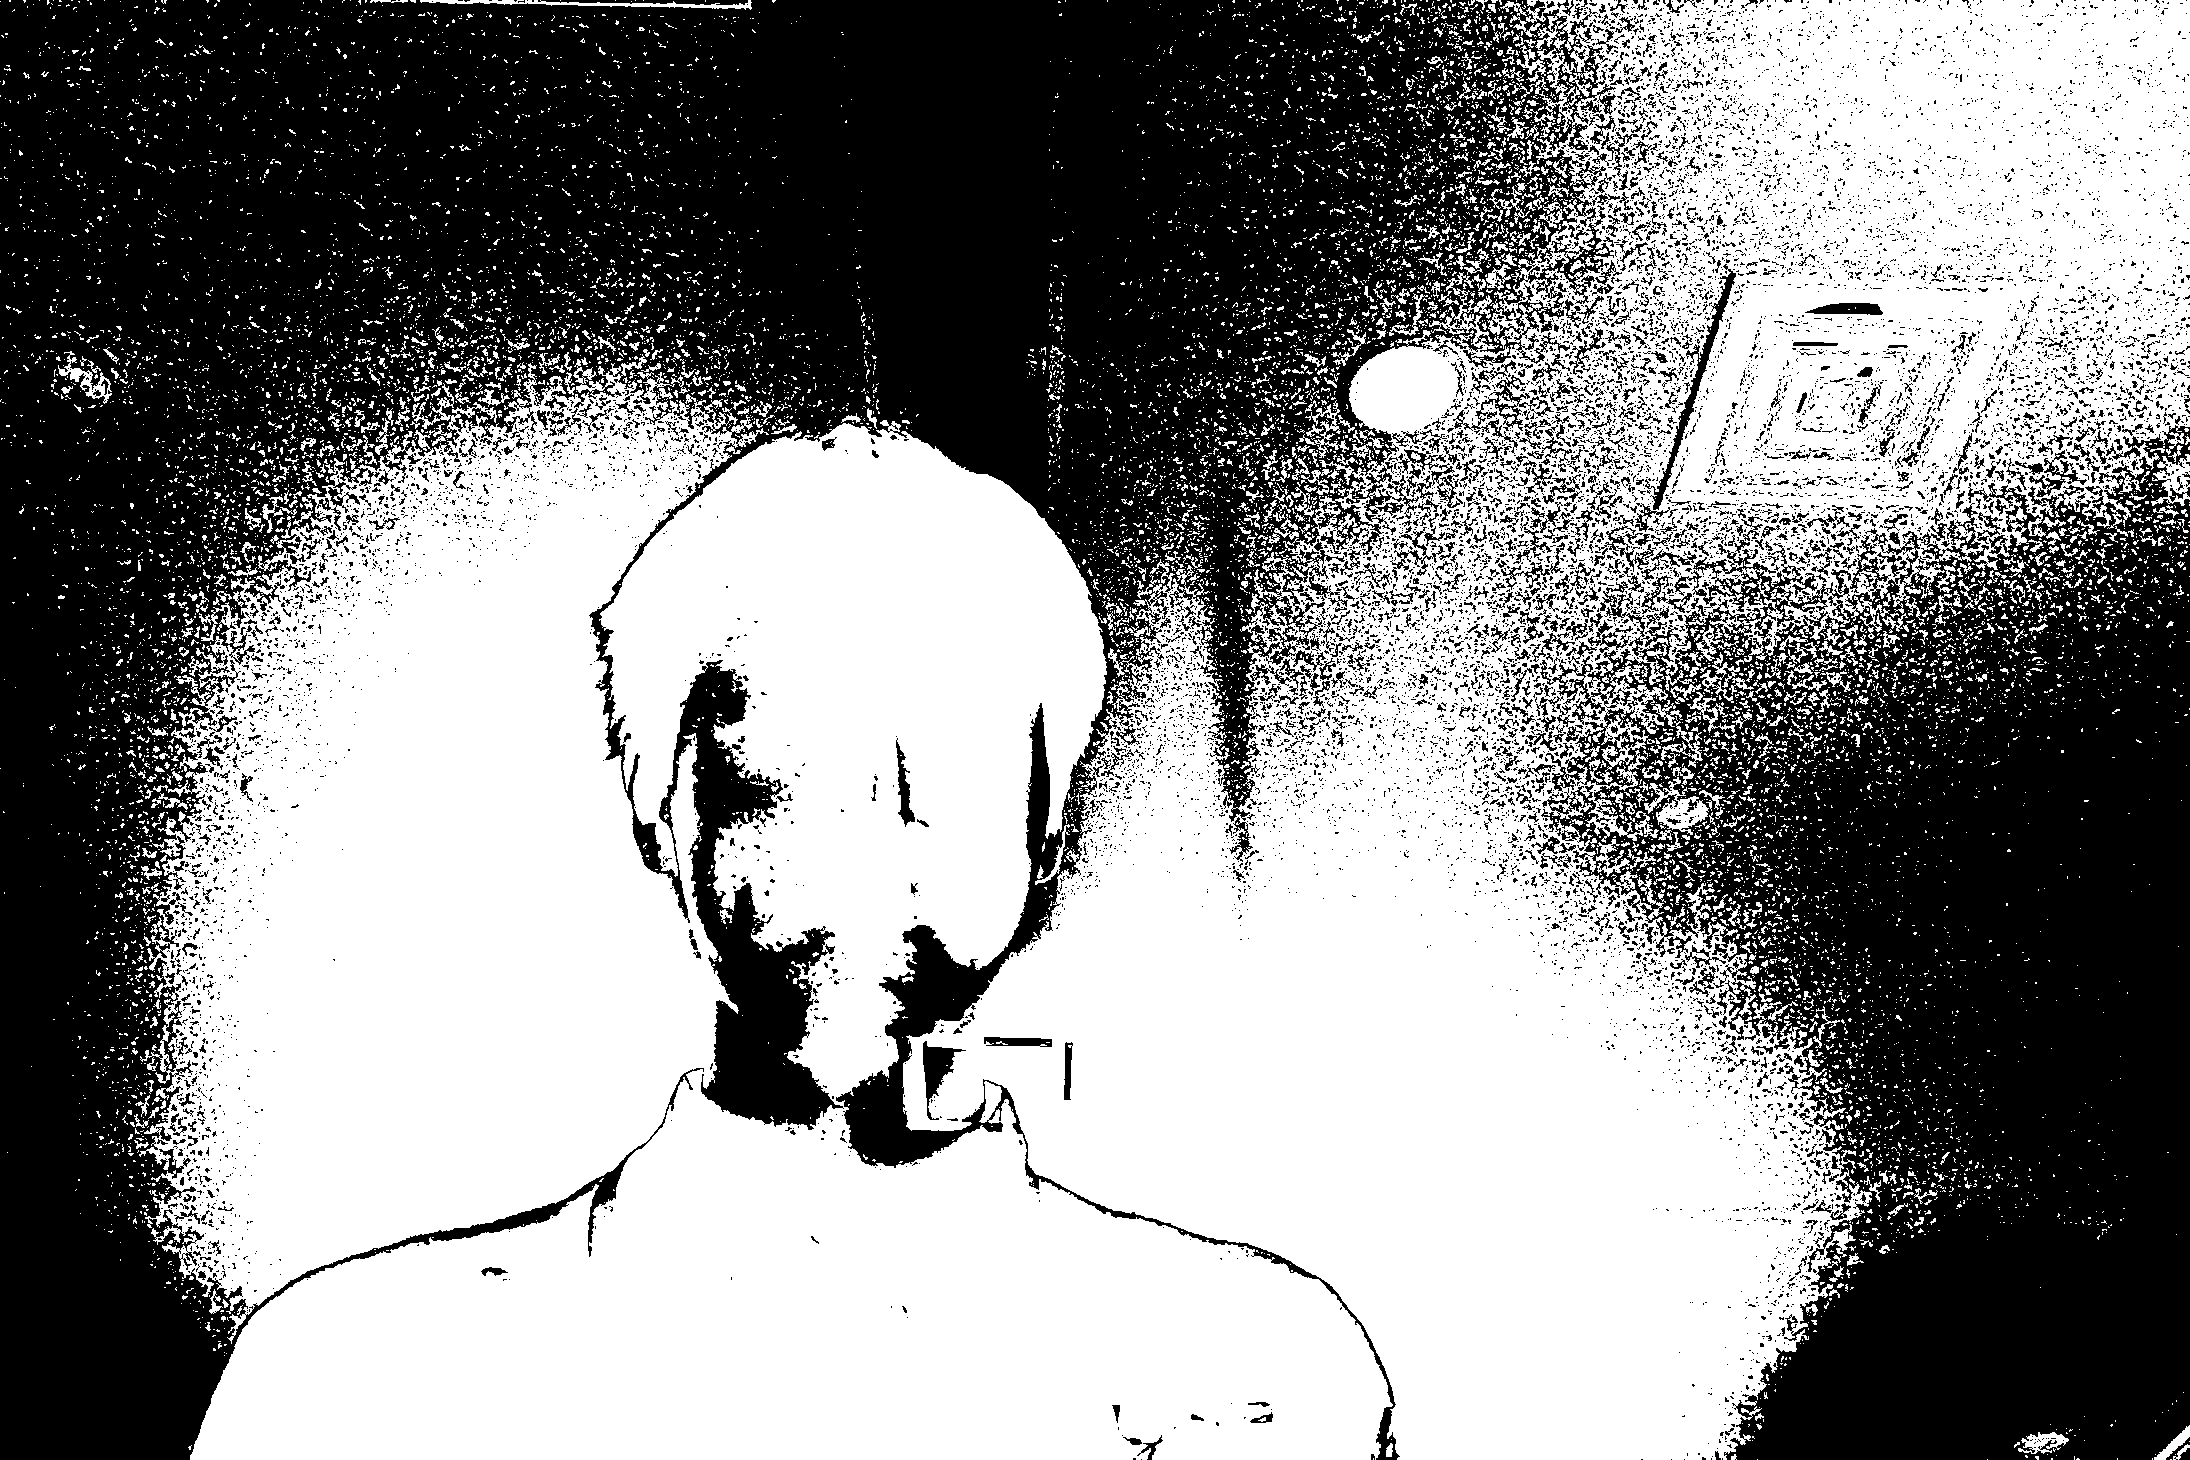
\includegraphics[keepaspectratio,width=\textwidth]{../../Figures/05_61.png}
            \subcaption{閾値\ \(32\)}
        \end{minipage}
        \begin{minipage}[b]{.3\textwidth}
            \centering
            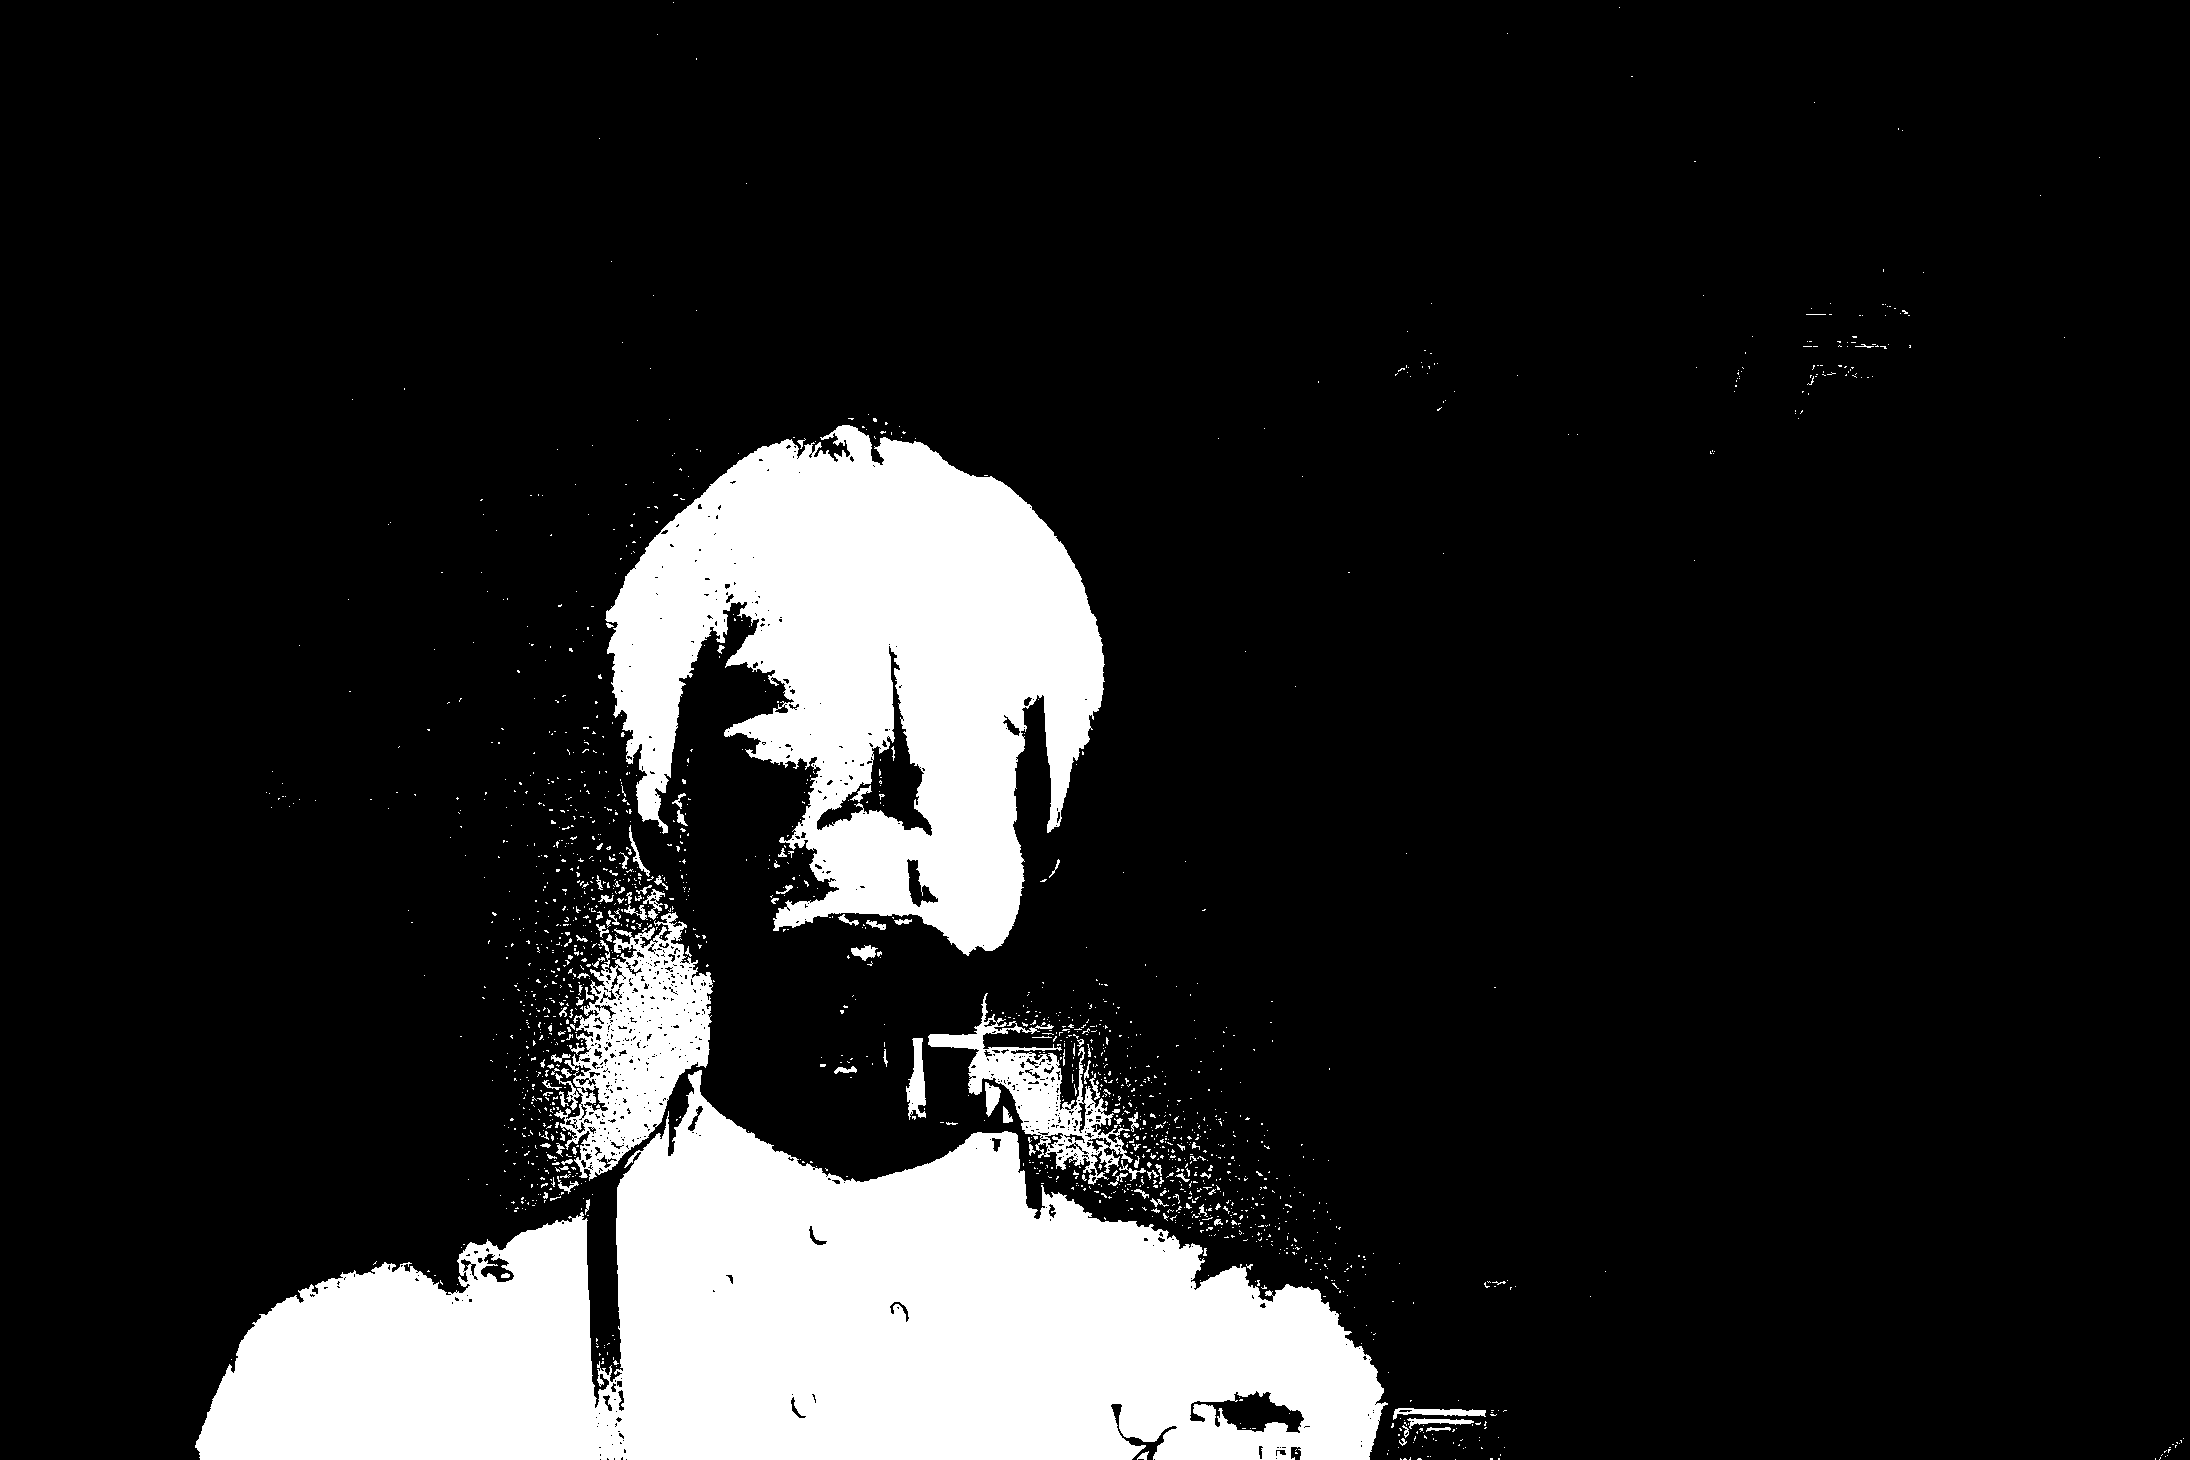
\includegraphics[keepaspectratio,width=\textwidth]{../../Figures/05_62.png}
            \subcaption{閾値\ \(64\)}
        \end{minipage}
        \begin{minipage}[b]{.3\textwidth}
            \centering
            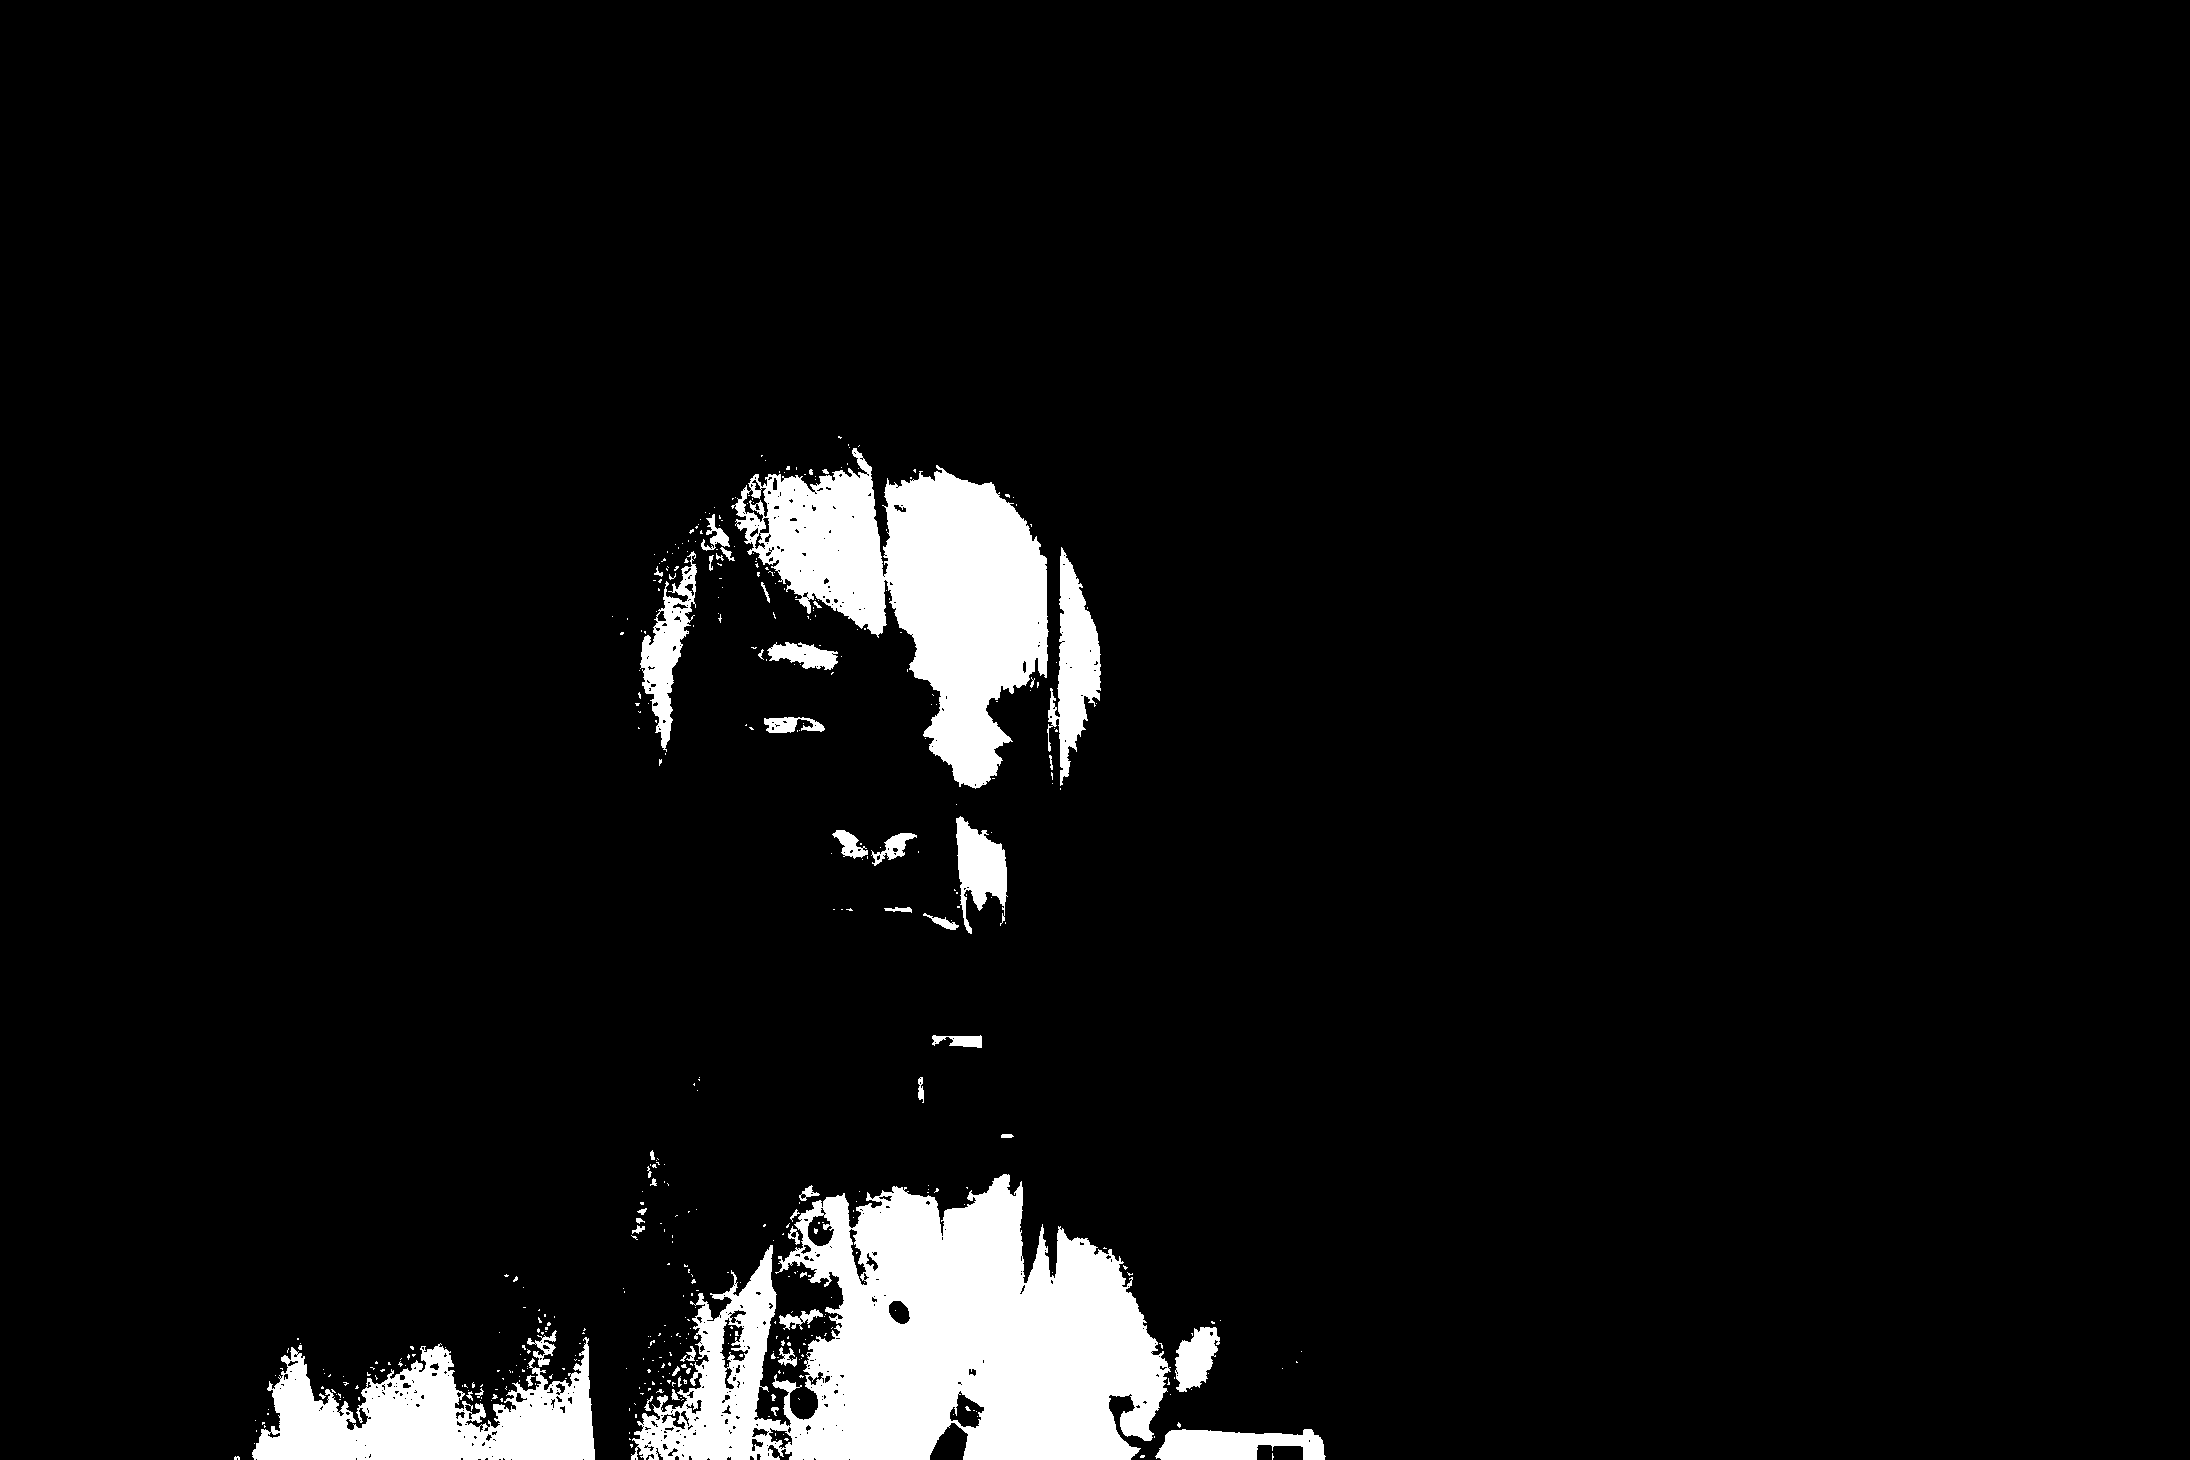
\includegraphics[keepaspectratio,width=\textwidth]{../../Figures/05_63.png}
            \subcaption{閾値\ \(128\)}
        \end{minipage}
        \caption{背景差分画像の閾値処理}
    \end{minipage}
\end{figure}
\footnotetext[1]{NTSC輝度信号のグレイスケール画像}
\section{\consideration}
\paragraph{\kadaiaa}
実験結果より,原画像に近い画像は,緑チャネルだけを抜き出してグレイスケール画像として表示したものである.
また,赤チャネルと青チャネルを入れ替えた画像では,文字や建物の概形を,はっきりとらえることができる.
これらは,\eqref{equ:grayscale}でGreenの割合が一番多い理由と考えられる.
\paragraph{\kadaiab}
量子化数を減らすことで,等高線のようなものが見える.
これは,元画像でなだらかな画素値の変化箇所が,量子化数を減らすことでとびとびの値になることで生じる.これを擬似輪郭という.
擬似輪郭は,量子化数を減らすことでより顕著になる.
\paragraph{\kadaiac}
量子化数が減ると擬似輪郭が生じる.この擬似輪郭は,階調反転しても変わらない.
\paragraph{\kadaiad}
閾値を調節することで,擬似輪郭を境に白と黒に別れることがわかった.
\paragraph{\kadaiaf}
背景差分画像では,被写体がぼんやりと写っている.この画像に対して閾値処理することで,被写体を強調できることが分かった.

\chapter{\kadaib}
\section{\purpose}
この実験では,画像に対してフィルタの適用や色空間を変換する.\par
\paragraph{画像フィルタ} 画像に対して,フィルタを適用するとはどのようなことか?我々は,携帯電話の写真アプリケーションを用いて,写真を「加工」する.
我々は「加工」という行為を「フィルタをかける」と呼ぶが,この「フィルタ」という言葉と,画像処理におけるフィルタは意味が異なる.
画像処理におけるフィルタは,画像ないに含まれる雑音を除去したり,特徴を抽出したりすることで欠陥検出をより円滑に行うための基本処理を指す\cite{画像フィルタ}.
\newcommand{\originimg}{\texttt{original\_img}}
\newcommand{\wgnimg}{\texttt{wgn\_img}}
\newcommand{\inimg}{\texttt{in\_img}}
テスト画像として,以下の画像を用意する.グレイスケール元画像を\originimg とする.
\begin{enumerate}
    \item \textbf{白色ガウス雑音}\\
          白色ガウス雑音は,白色性を持つガウス雑音である.今回は,平均\(0\),標準偏差\(10\)としてガウス分布の乱数を発生させる.
          このテスト画像を\wgnimg とする.
    \item \textbf{インパルス雑音}\\
          インパルス雑音とは.超短時間におこる高周波の雑音のことを指す.今回は,画像のランダムな画素を,白または黒で塗り替える.それぞれ全体画素の1\(\%\) の割合で作成する.
          このテスト画像を\inimg とする.
\end{enumerate}
画像フィルタはいくつかの種類があり,画像雑音の除去やエッジの強調に用いられる.
\begin{enumerate}
    \item \textbf{平滑化フィルタ}
          \begin{itemize}
              \item 画像の各画素\(p\)に対して,\(n\)近傍と中央の画素値の平均や重み付け平均をとり,\(p\)の画素値とするフィルタ.
              \item 今回の実験では,各画素\(p\)に対して,\(3\times 3\),つまり8近傍と\(p\)の画素値の平均をとり,中央の画素値として定義する.2つのテスト画像にフィルタを適用し,雑音とフィルタの関係を考察する.
          \end{itemize}
    \item \textbf{メディアンフィルタ}
          \begin{itemize}
              \item 画像の各画素\(p\)に対して,\(n\)近傍と中央の画素値を昇順に整列し,その中央値を\(p\)の画素値とする.
              \item 今回の実験では,各画素\(p\)に対して,\(3\times 3\),つまり8近傍と\(p\)の画素値を昇順に整列する.その中央値を\(p\)の画素値として定義する.2つのテスト画像にフィルタを適用し,雑音とフィルタの関係を考察する.
          \end{itemize}
    \item \textbf{微分フィルタ}
          \begin{itemize}
              \item 微分フィルタは,境界線の強調や局所的な特徴の抽出するフィルタである.しかし,一次微分フィルタ,二次微分フィルタを用いると,画像の雑音も強調される.ここでPrewittフィルタとSobelフィルタを用いると,雑音がある画像でもうまく境界線を抽出できる\cite[p.87]{画像処理}.
                    \begin{itemize}
                        \item \textbf{Prewitt フィルタ}:隣り合う2画素の画素値を持ちいて3画素ずつをセットにして濃度の変化点を抽出するアルゴリズム\cite[p.87]{画像処理}.
                        \item \textbf{Sobel フィルタ}:画像の各ピクセルの周囲の画素との差を計算して,その差の大きさを使って,エッジを検出するアルゴリズム.
                    \end{itemize}
              \item 今回の実験では,\originimg に対して,Sobelフィルタを用いて縦微分,横微分,縦微分と横微分の加算合成した画像を作成する.フィルタを適用した画像の特徴と,それぞれの違いを考察する.
          \end{itemize}
    \item \textbf{Laplacianフィルタ}
          \begin{itemize}
              \item Laplacianフィルタは,微分フィルタ同様,境界線を見つけるために使われる方法である.
              \item 今回の実験では,\originimg に対して,Laplacianフィルタを適用し,閾値処理する.フィルタを適用し閾値処理した画像と特徴と違いを考察する.
          \end{itemize}
\end{enumerate}
\begin{figure}[h]
    \centering
    \begin{minipage}[b]{.24\textwidth}
        \centering
        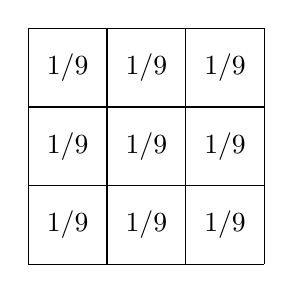
\begin{tikzpicture}
            \draw (0,0) grid (3,3);
            \foreach \u \v in {0.5/0.5,1.5/0.5,2.5/0.5,0.5/1.5,1.5/1.5,2.5/1.5,0.5/2.5,1.5/2.5,2.5/2.5}
            \node at (\u,\v) {\(1/9\)};
        \end{tikzpicture}
        \subcaption{平滑化フィルタ}
        \label{fig:平滑化フィルタ}
    \end{minipage}
    \begin{minipage}[b]{.24\textwidth}
        \centering
        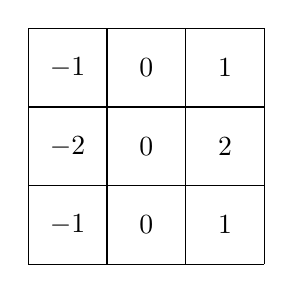
\begin{tikzpicture}
            \draw (0,0) grid (3,3);
            \foreach \u \v \w in {0.5/0.5/{\(-1\)},1.5/0.5/{\(0\)},2.5/0.5/{\(1\)},0.5/1.5/{\(-2\)},1.5/1.5/{\(0\)},2.5/1.5/{\(2\)},0.5/2.5/{\(-1\)},1.5/2.5/{\(0\)},2.5/2.5/{\(1\)}}
            \node at (\u,\v) {\w};
        \end{tikzpicture}
        \subcaption{Prewittフィルタ:横方向}
        \label{fig:Prewittフィルタ_横方向}
    \end{minipage}
    \begin{minipage}[b]{.24\textwidth}
        \centering
        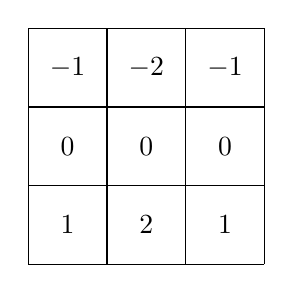
\begin{tikzpicture}
            \draw (0,0) grid (3,3);
            \foreach \u \v \w in {0.5/0.5/{\(1\)},1.5/0.5/{\(2\)},2.5/0.5/{\(1\)},0.5/1.5/{\(0\)},1.5/1.5/{\(0\)},2.5/1.5/{\(0\)},0.5/2.5/{\(-1\)},1.5/2.5/{\(-2\)},2.5/2.5/{\(-1\)}}
            \node at (\u,\v) {\w};
        \end{tikzpicture}
        \subcaption{Prewittフィルタ:縦方向}
        \label{fig:Prewittフィルタ_縦方向}
    \end{minipage}
    \begin{minipage}[b]{.24\textwidth}
        \centering
        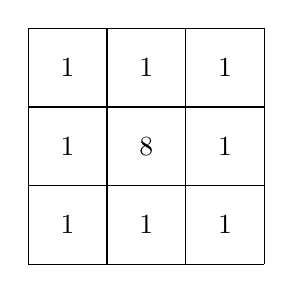
\begin{tikzpicture}
            \draw (0,0) grid (3,3);
            \foreach \u \v in {0.5/0.5,1.5/0.5,2.5/0.5,0.5/1.5,2.5/1.5,0.5/2.5,1.5/2.5,2.5/2.5}
            \node at (\u,\v) {\(1\)};
            \node at (1.5,1.5) {\(8\)};
        \end{tikzpicture}
        \subcaption{Laplacianフィルタ}
        \label{fig:Laplacianフィルタ}
    \end{minipage}
    \caption{\(3\times 3\)画像フィルタ}
\end{figure}
\paragraph{色空間変換}この実験では,RGB色空間から,HSV色空間へ変換する.RGB色空間は,赤(Red),緑(Green),青(Blue)の3チャネルで構成する.HSVは色相(Hue),彩度(Saturation),明度(Value)の3チャネルで構成する.
色相は,カラー ホイール上の色の位置に対応する,\(0\)から\(100\)の値,色相の量または中間からの逸脱.特定の色の赤,緑,青成分の中での最大値.いずれも\texttt{double}型で保存される\cite{rgb2hsv}.
HSV色空間の特徴として,人間が色を知覚する方法と類似しており,視覚障害者向けのアクセシビリティ向上に役立つことが挙げられる.たとえば,HSVの「明度」を調節することで,文字が見やすくなる\cite[p.97\ -\ p.98]{画像処理}.
また,人間が色を知覚する方法と類似していることを踏まえて,HSV色空間を用いることで,画像の特徴を抽出しやすくなる.
今回の実験では,自分の手の写真をRGB色空間からHSV色空間へ変換し,肌色領域を抽出する.抽出した肌色領域を白色,そのほかの部分を黒色にして出力する.出力した画像と,RGB色空間における肌色領域を抽出した場合の精度について考察する.

\begin{wrapfigure}{r}[0mm]{.3\textwidth}
    \vspace{-.5cm}
    \begin{lstlisting}[caption={白色ガウス雑音画像の生成},label={src:白色ガウス雑音画像の生成}]
% 画像サイズ : n x m
wgn = 10*randn(n, m);
wgn = uint8(wgn);
wgn_img = wgn + gimg;
    \end{lstlisting}
    \begin{lstlisting}[caption={インパルス雑音画像の生成},label={src:インパルス雑音画像の生成}]
% 画像サイズ : n x m
rnd = rand(n, m);
b = (rnd < 0.01);
w = (rnd > 0.99);
in_img(w) = 255;
in_img(b) = 0;
    \end{lstlisting}
    \vspace{-1cm}
\end{wrapfigure}
\section{\method}
\paragraph{白色ガウス雑音を加えた画像}
白色ガウス雑音の作成には\texttt{randn}関数を用い,生成した乱数と,標準偏差の積を取る.生成した乱数を\texttt{uint8}型に変換し,\originimg と和を取る(\srcref{src:白色ガウス雑音画像の生成}).
\(255\)を上回る,または\(0\)を下回る場合,それぞれの値に変換したものを, \wgnimg とする.
\paragraph{インパルス雑音を加えた画像}
インパルス雑音は,\texttt{rand}関数を用いて作成する.発生率を\(1\%\) にするため,乱数の\(0.01\)未満の画素を黒,乱数の\(0.99\)より大きい画素を白としてインパルスノイズを設計する(\srcref{src:インパルス雑音画像の生成}).
\paragraph{フィルタの適用}
平滑化フィルタ,微分フィルタ,Laplacianフィルタの適用は,\texttt{filter2}関数,(\ \verb|filter2(filter, img)|\ )を用いる.
メディアンフィルタは,画像の\mat{i}{j}に対して,\texttt{median}関数を用いてフィルタ処理する.メディアンフィルタを適用する際に,四方に画素がない画素(\mat{1}{1}画素,\mat{m}{1}画素など)はフィルタ処理できないため,0パディング処理を行い,メディアンフィルタを適用する(\srcref{src:メディアンフィルタの適用}).
\begin{lstlisting}[caption={メディアンフィルタの適用},label={src:メディアンフィルタの適用},frame={left}]
for h = 2:img_height % 画像行列 img の高さ
    for w = 2:img_width % 画像行列 img の横幅,median_filter は0パディング後のimg
        median_filter(h-1, w-1) = median(img(h-1:h+1,w-1:w+1),"all"); 
    end
end
\end{lstlisting}
課題(フィルタ処理)のスクリプトは,\sref{src:06_01} - \sref{src:06_04}.
\paragraph{色空間変換}
読み込んだ画像はRGB色空間で保存される.この画像をHSV色空間に変換するためには,\texttt{rgb2hsv}関数を用いる.
出力された値と\(255\)の積を取り,HSV色空間で出力された画像を書き出す.
色相,彩度,明度それぞれのチャネルを抽出し,\matlab のアプリケーションを用いて,肌色要素のHSV成分を出力する(\sref{src:06_05_f}).
それぞれの値に合致した画素を,画素値\(255\),ほかの画素値を\(0\)とした画像を書き出す.同様な方法で,RGB色空間における肌色領域の抽出も行う(\sref{src:06_05_f2}).
\scall{\kadaibe}\sref{src:06_05},\sref{src:06_05_1}.
\section{\result}
\begin{figure}[h]
    \centering
    \begin{minipage}[b]{.3\textwidth}
        \centering
        
\includegraphics[keepaspectratio,width=\textwidth]{../../Figures/05_21_gimg.png}
        \subcaption{元画像}
    \end{minipage}
    \begin{minipage}[b]{.3\textwidth}
        \centering
        
\includegraphics[keepaspectratio,width=\textwidth]{../../06_ImageFiltering/file_white-Gaussian-Noise.png}
        \subcaption{白色ガウス雑音(\wgnimg)}
    \end{minipage}
    \begin{minipage}[b]{.3\textwidth}
        \centering
        
\includegraphics[keepaspectratio,width=\textwidth]{../../06_ImageFiltering/file_impluse-noise.png}
        \subcaption{インパルス雑音(\inimg)}
    \end{minipage}
    \caption{\kadaiaa\ 実験結果}
    \begin{minipage}[b]{.49\textwidth}
        \begin{minipage}[b]{.49\textwidth}
            
\includegraphics[keepaspectratio,width=\textwidth]{../../Figures/06_21_sf_img_wgn.png}
            \subcaption{\wgnimg}
        \end{minipage}
        \begin{minipage}[b]{.49\textwidth}
            
\includegraphics[keepaspectratio,width=\textwidth]{../../Figures/06_22_sf_img_in.png}
            \subcaption{\inimg}
        \end{minipage}
        \caption{平滑化フィルタ}
    \end{minipage}
    \begin{minipage}[b]{.49\textwidth}
        \begin{minipage}[b]{.49\textwidth}
            
\includegraphics[keepaspectratio,width=\textwidth]{../../Figures/06_23_mf_img_wgn.png}
            \subcaption{\wgnimg}
        \end{minipage}
        \begin{minipage}[b]{.49\textwidth}
            
\includegraphics[keepaspectratio,width=\textwidth]{../../Figures/06_24_mf_img_in.png}
            \subcaption{\inimg}
        \end{minipage}
        \caption{メディアンフィルタ}
    \end{minipage}
    \begin{minipage}[b]{.3\textwidth}
        \centering
        
\includegraphics[keepaspectratio,width=\textwidth]{../../Figures/06_31_diff-x-img.png}
        \subcaption{横方向Sobelフィルタ}
    \end{minipage}
    \begin{minipage}[b]{.3\textwidth}
        \centering
        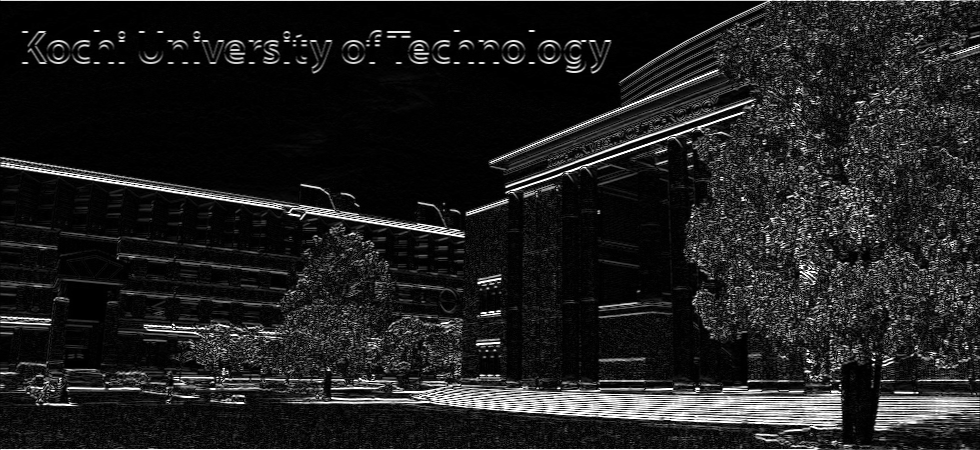
\includegraphics[keepaspectratio,width=\textwidth]{../../Figures/06_32_diff-y-img.png}
        \subcaption{縦方向Sobelフィルタ}
    \end{minipage}
    \begin{minipage}[b]{.3\textwidth}
        \centering
        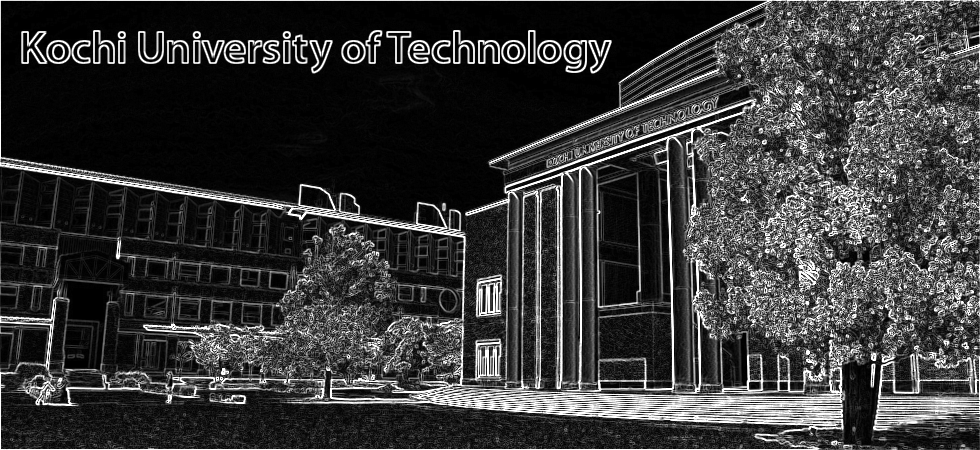
\includegraphics[keepaspectratio,width=\textwidth]{../../Figures/06_33_diff-img.png}
        \subcaption{Sobelフィルタ\footnotemark}
    \end{minipage}
    \caption{Sobelフィルタ適用}
    \begin{minipage}[b]{.3\textwidth}
        \centering
        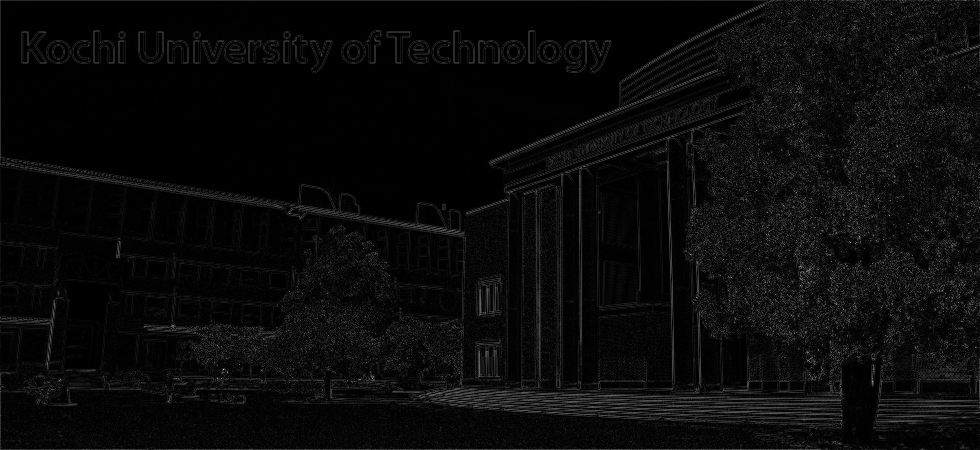
\includegraphics[keepaspectratio,width=\textwidth]{../../Figures/06_41_lf-img}
        \subcaption{Laplacianフィルタ}
    \end{minipage}
    \begin{minipage}[b]{.3\textwidth}
        \centering
        
\includegraphics[keepaspectratio,width=\textwidth]{../../Figures/06_43_lf-img-thresholding.png}
        \subcaption{閾値処理\ \((=30)\)}
    \end{minipage}
    \begin{minipage}[b]{.3\textwidth}
        \centering
        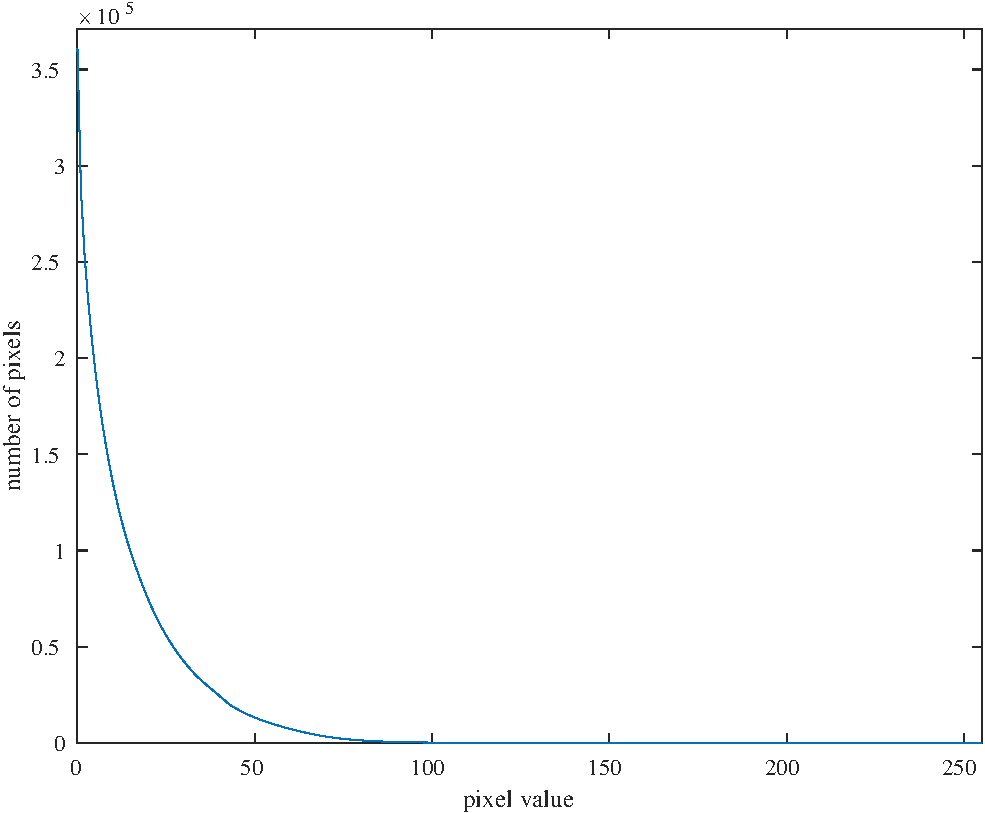
\includegraphics[keepaspectratio,width=\textwidth]{../../Figures/06_42_Thresholding-graph.pdf}
        \subcaption{画素値ヒストグラム}
        \label{fig:Laplacianフィルタのヒストグラム}
    \end{minipage}
    \caption{Laplacianフィルタの適用と処理}
\end{figure}
\footnotetext{横方向Sobelフィルタ適用後画像と縦方向Sobelフィルタ適用後画像の和.}
\begin{figure}[ht]
    \centering
    \begin{minipage}[b]{.23\textwidth}
        \centering
        \includegraphics[keepaspectratio,width=\textwidth]{../../06_ImageFiltering/file_hand.png}
        \subcaption{元画像}
    \end{minipage}
    \begin{minipage}[b]{.23\textwidth}
        \centering
        \includegraphics[keepaspectratio,width=\textwidth]{../../Figures/06_51_img-hsv.png}
        \subcaption{HSV色空間への変換後}
    \end{minipage}
    \begin{minipage}[b]{.23\textwidth}
        \centering
        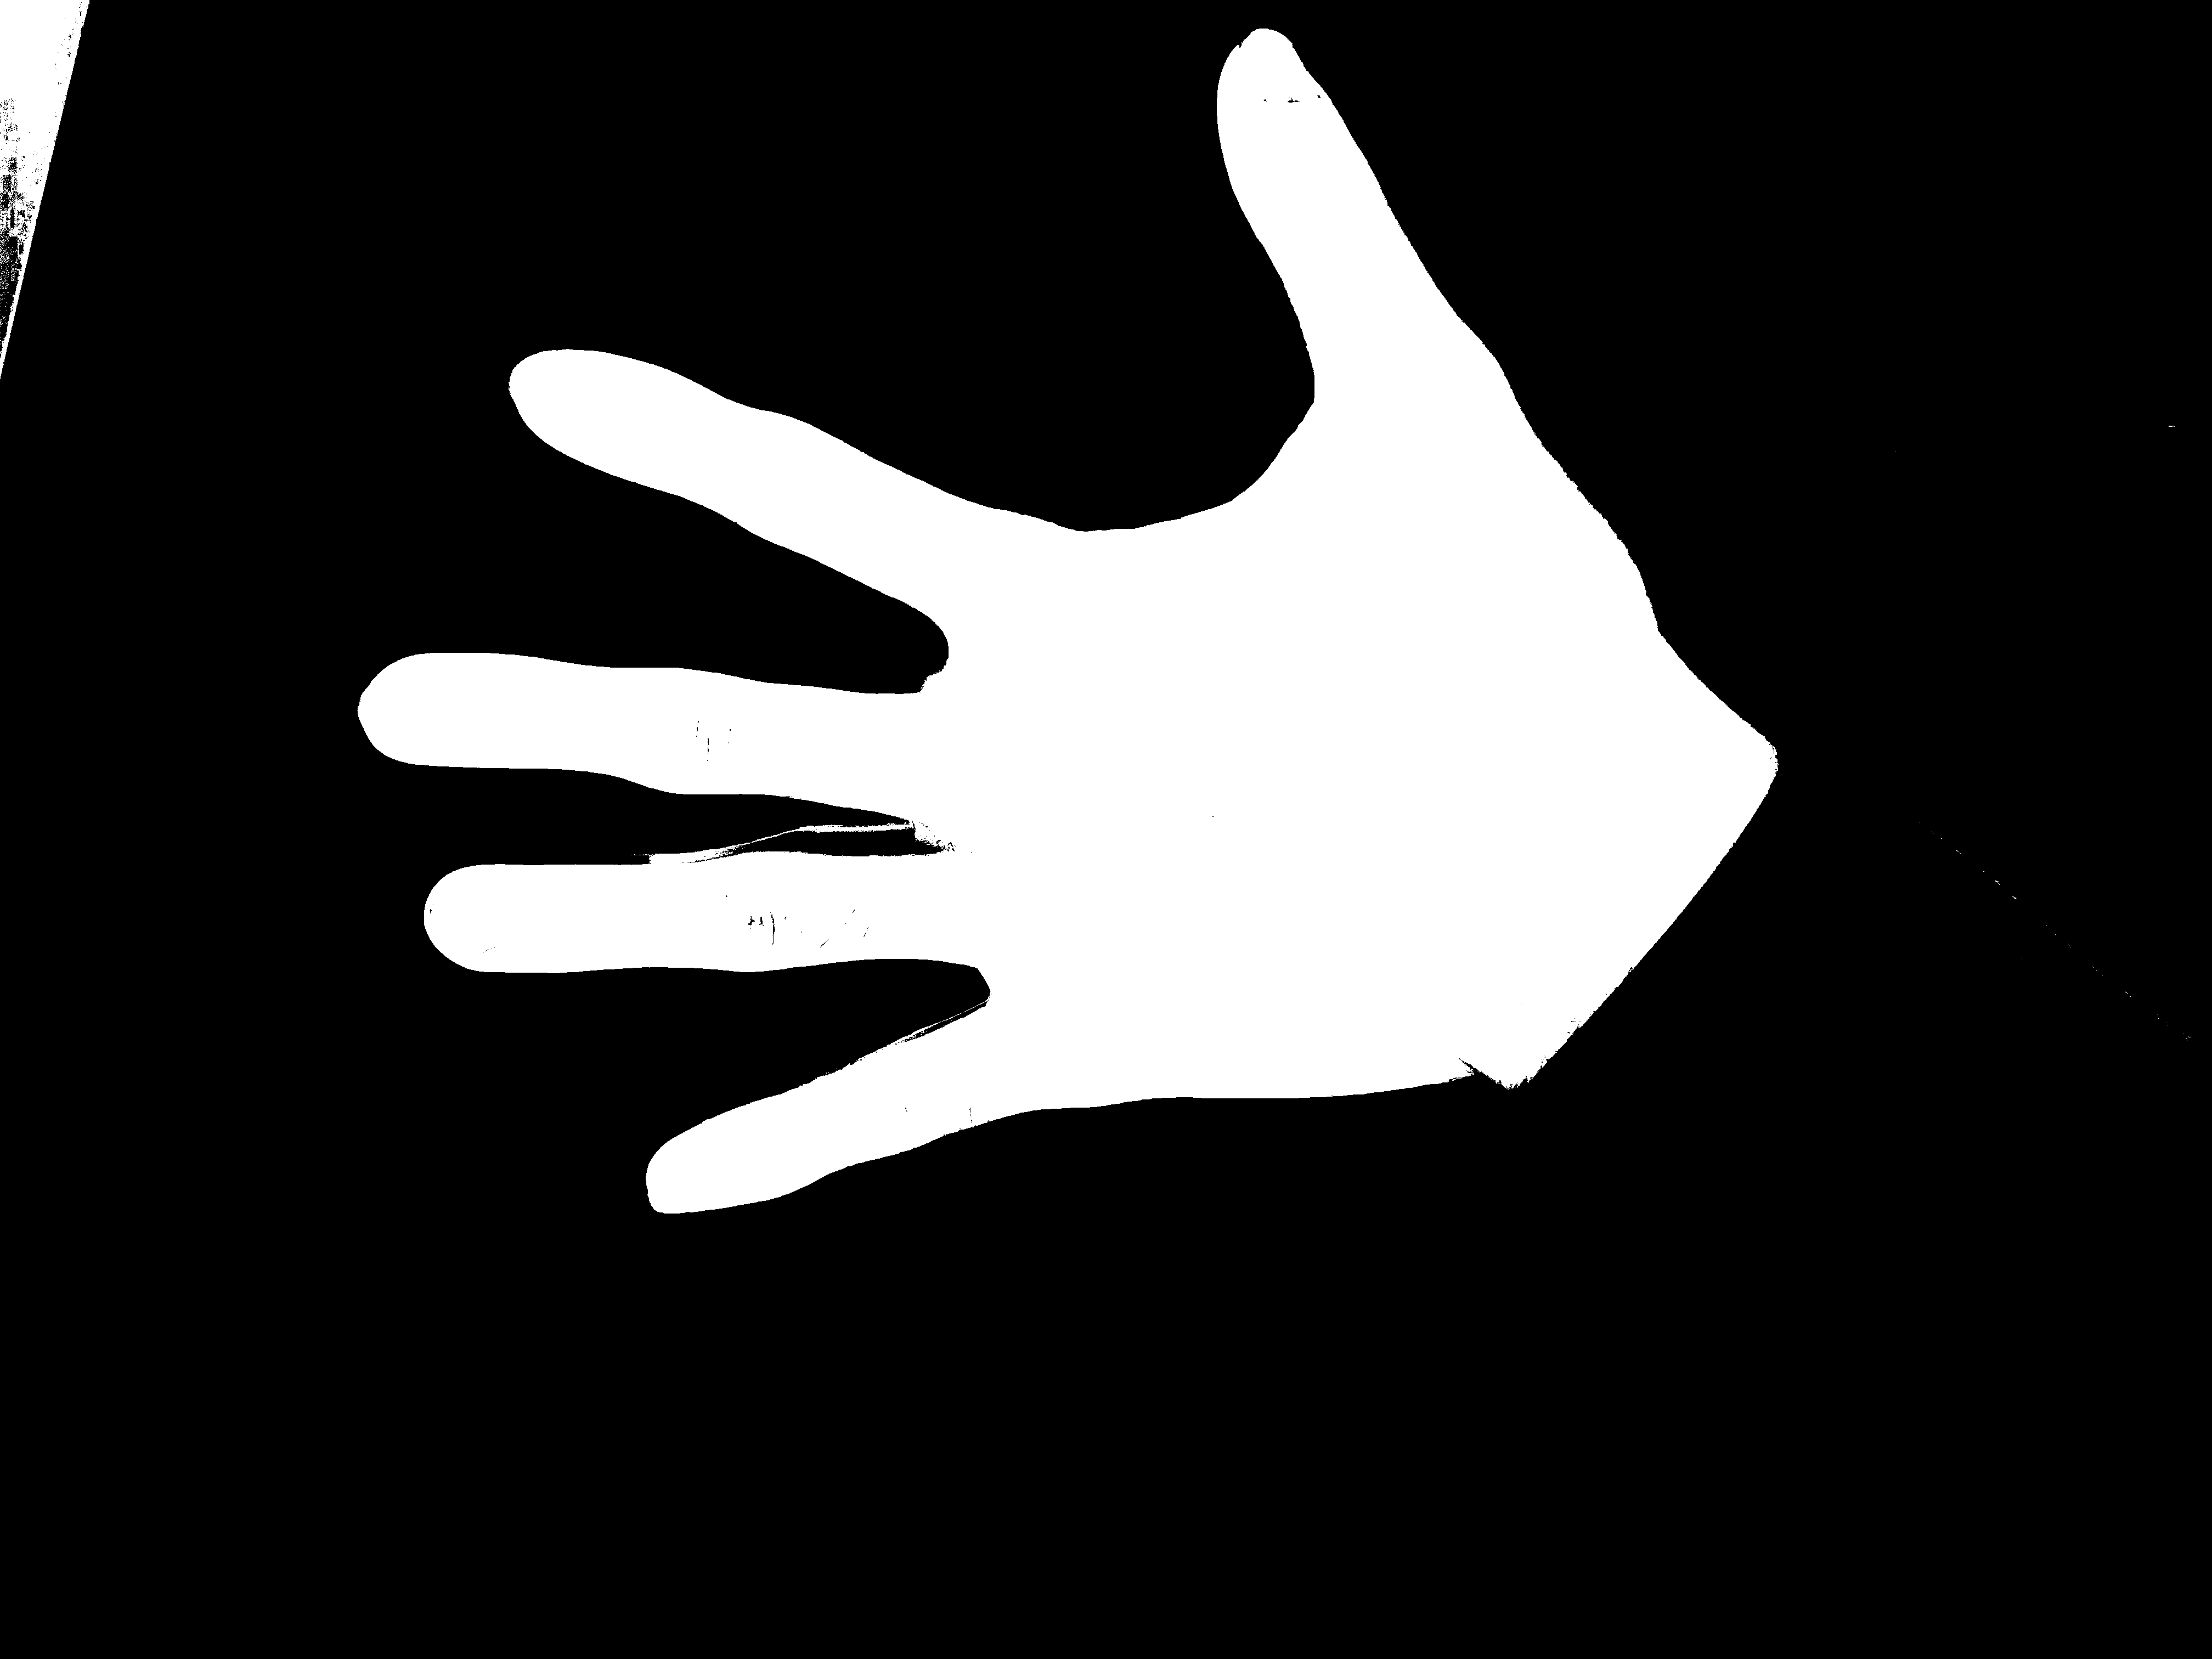
\includegraphics[keepaspectratio,width=\textwidth]{../../Figures/06_52_scd.png}
        \subcaption{肌色領域の抽出(HSV)}
    \end{minipage}
    \begin{minipage}[b]{.23\textwidth}
        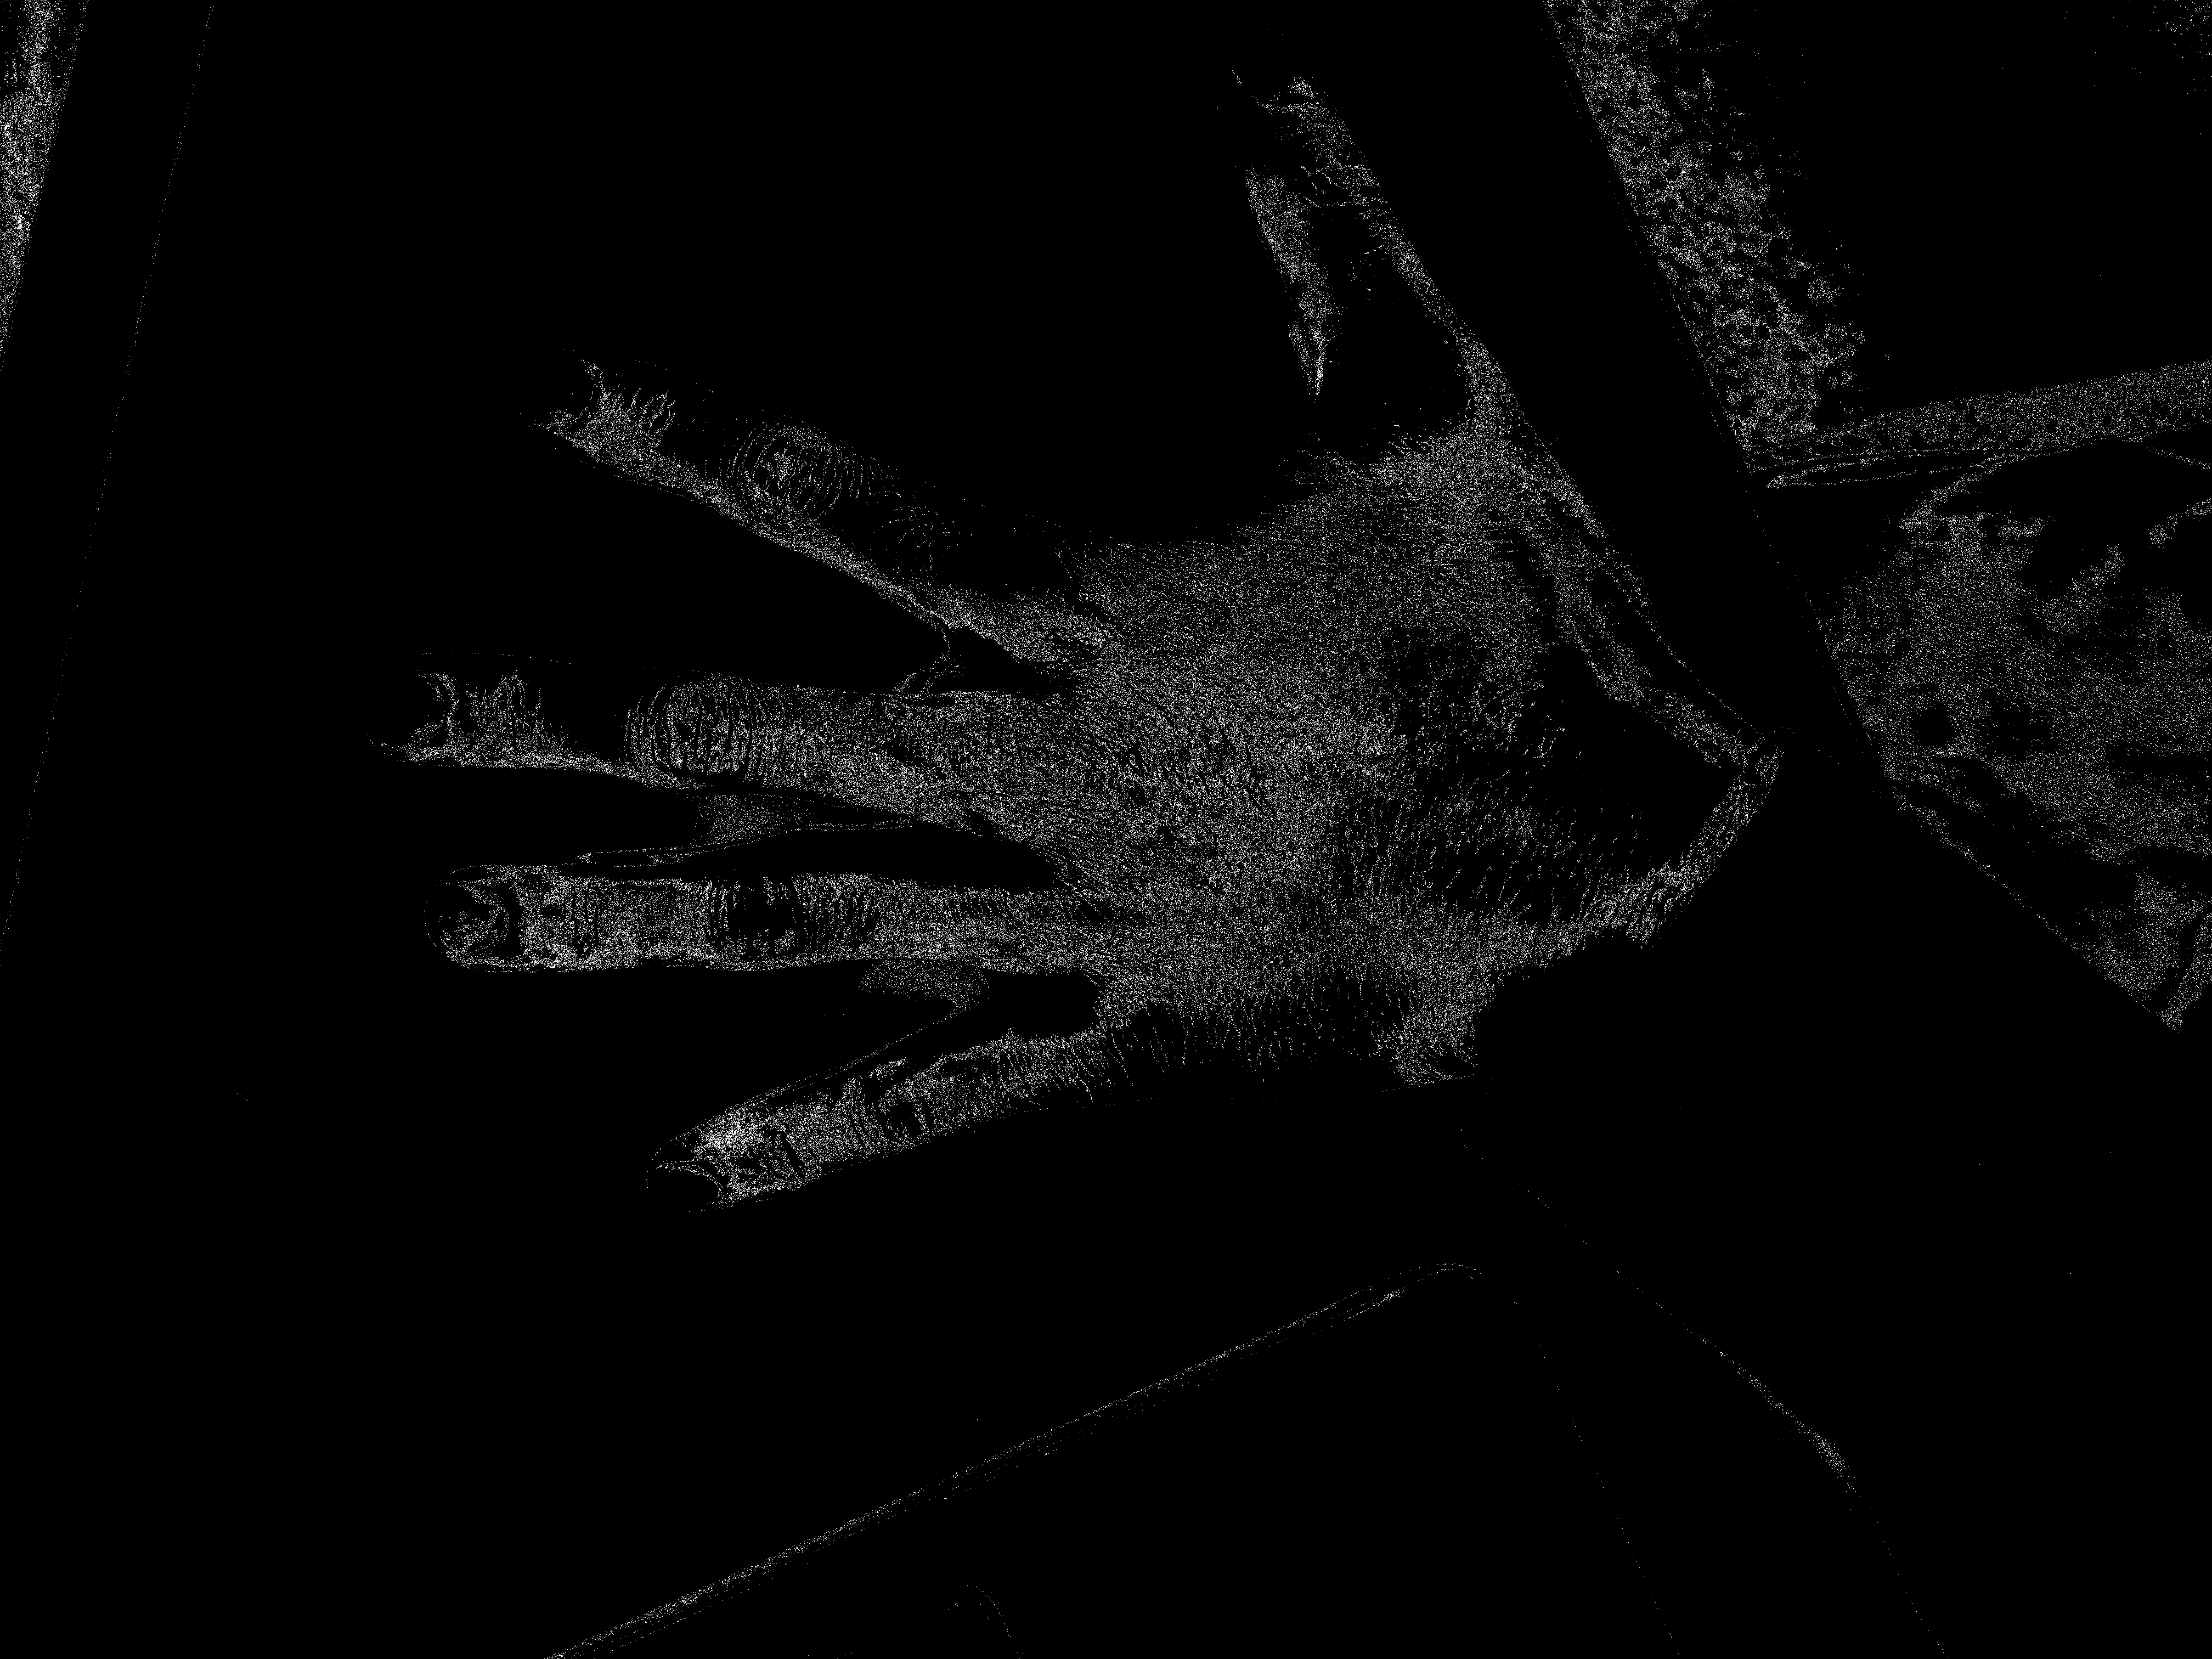
\includegraphics[keepaspectratio,width=\textwidth]{../../Figures/06_53_hand.png}
        \subcaption{肌色領域の抽出(RGB)}
    \end{minipage}
    \caption{\kadaibe\ 実験結果}
\end{figure}
\paragraph{平滑化フィルタ,メディアンフィルタ}
\wgnimg に対して平滑化フィルタを適用すると,雑音部分が目立たなくなった.また,\inimg に対して平滑化フィルタを適用すると,雑音が取り除かれることなく残った.
\wgnimg と\inimg に対してメディアンフィルタを適用すると,雑音部分が目立たなくなった.
\paragraph{Sobelフィルタ,Laplacianフィルタ}
横微分フィルタを適用すると,縦方向のエッジが強調され,縦方向微分フィルタを適用すると,横方向のエッジが強調された.
これらの画像を足し合わせて,\(255\)を上回る値を処理すると,画像全体のエッジが強調された画像を生成できた.
Laplacianフィルタを適用すると,画像が暗く出力された.この画像に対して\figref{fig:Laplacianフィルタのヒストグラム}を用いて,閾値\(30\)の閾値処理し,全体画像のエッジが強調された画像を生成できた.
\section{\consideration}
\paragraph{Sobelフィルタ,メディアンフィルタ}
メディアンフィルタは,ノイズに強いことがわかる.これは中央値を算出することにより,ノイズでない値が中央値となるからである.
ただし,画素値の中央値を抽出するため,平均値を算出する平滑化フィルタに比べて,計算量が多い.
それに対して,平滑化フィルタは,ノイズの画素値を含めた値の平均を算出するので,メディアンフィルタに比べるとノイズに弱い.
\paragraph{Sobelフィルタ,Laplacianフィルタ}
Sobelフィルタは,画像の隣接画素間の差分を計算する.よって,差が激しい画素の画素値が大きくなり,白く表示される.
つまり,ノイズに対してもエッジが強調される.
Laplacianフィルタは,画像の二次微分を計算することでエッジの位置を抽出している.Laplacianフィルタは高周波成分を増幅するため,ノイズに対してもエッジが強調される.
\paragraph{色空間変換}
HSV色空間での肌色領域の方が,RGB色空間での肌色領域よりも,明らかに正確である.
RGB色空間では,明暗(影や光の状況)でRGB値が変わるのに対して,HSV色空間では,明暗が「明度」というチャネルで保存されているので,光の状況や影に左右されず,肌色領域をより正確に抽出できる.
\bibliography{bib}
\chapter*{付録}
\pagestyle{appendixstyle}
\addcontentsline{toc}{chapter}{付録}
\setcounter{section}{0}
\renewcommand{\thelstlisting}{\thesection-\arabic{lstlisting}}
\renewcommand{\thesection}{\Alph{section}}
\newcommand{\secref}[1]{[#1]{#1}}
\makeatletter
\@addtoreset{lstlisting}{section}
\makeatother
\lstset{
    frame={single},
    numbers={left}
}
\section{\kadaia\ (April 27th, 2023)}
\lstinputlisting[caption={\secref{\kadaiaa}},label={src:05_01}]{../../05_UnderstandingImages/no1.m}
\lstinputlisting[caption={\secref{\kadaiab}},label={src:05_02}]{../../05_UnderstandingImages/no2.m}
\lstinputlisting[caption={\secref{\kadaiac}},label={src:05_03}]{../../05_UnderstandingImages/no3.m}
\lstinputlisting[caption={\secref{\kadaiad}},label={src:05_04}]{../../05_UnderstandingImages/no4.m}
\lstinputlisting[caption={\secref{\kadaiae}},label={src:05_05}]{../../05_UnderstandingImages/no5.m}
\lstinputlisting[caption={\secref{\kadaiaf}},label={src:05_06}]{../../05_UnderstandingImages/no6.m}
\section{\kadaib\ (May 8th, 2023)}
\lstinputlisting[caption={\secref{\kadaiba}},label={src:06_01}]{../../06_ImageFiltering/no1.m}
\lstinputlisting[caption={\secref{\kadaibb}},label={src:06_02}]{../../06_ImageFiltering/no2.m}
\lstinputlisting[caption={\secref{\kadaibc}},label={src:06_03}]{../../06_ImageFiltering/no3.m}
\lstinputlisting[caption={\secref{\kadaibd}},label={src:06_04}]{../../06_ImageFiltering/no4.m}
\lstinputlisting[caption={\secref{\kadaibe}},label={src:06_05}]{../../06_ImageFiltering/no5.m}
\lstinputlisting[caption={\secref{\kadaibd}\ \texttt{fucntion}},label={src:06_05_f}]{../../06_ImageFiltering/no5_hsvfunc.m}
\section{\ (April 20th, 2023)}
\section{\ (April 24th, 2023)}
\end{document}